\section{Model and Training}
\label{sec:model}

\subsection{Model architecture}

The optimal stopping DP runs backward ($C_t$ depends on $C_{t+1}$), but the agent processes observations forward. A transformer with $L$ layers compresses at most $L$ backward steps per pass. Our solution: a \emph{chain-of-thought scratchpad} that explicitly unrolls the DP, one step per token. A 2-layer transformer can then execute arbitrarily long backward inductions.

At each decision step $t$, a sub-chain computes $V(t, n{-}2) \to \cdots \to V(t, t)$, producing decision output $V(t) := V(t,t) \approx C_t/M$. Each sub-chain conditions on observations $x_0, \ldots, x_t$ only. Total chain length: $n(n{-}1)/2$.

\begin{figure}[h]
\centering
\fbox{\begin{minipage}{0.9\textwidth}
\textbf{Sequence layout} ($n = 5$, 15 tokens):
\begin{center}
\small
\begin{tabular}{|c|c|c|c|c||c|c|c|c||c|c|c||c|c||c|}
\hline
$x_0$ & $x_1$ & $x_2$ & $x_3$ & $x_4$ & $V_{0,3}$ & $V_{0,2}$ & $V_{0,1}$ & $V_{0,0}$ & $V_{1,3}$ & $V_{1,2}$ & $V_{1,1}$ & $V_{2,3}$ & $V_{2,2}$ & $V_{3,3}$ \\
\hline
\multicolumn{5}{|c||}{observations} & \multicolumn{4}{c||}{sub(0)} & \multicolumn{3}{c||}{sub(1)} & \multicolumn{2}{c||}{sub(2)} & sub(3) \\
\hline
\end{tabular}
\end{center}
Decision outputs (diagonal): $V_{0,0}, V_{1,1}, V_{2,2}, V_{3,3}$. Stop at first $t$ where $x_t \ge V(t) \cdot M$.
\end{minipage}}
\caption{2D chain-of-thought sequence layout.}
\label{fig:layout}
\end{figure}

\textbf{Architecture:} 2 layers (minimum for Bellman backup: FFN computes ReLU terms, attention computes PMF-weighted sum), 2 heads, $d_{\mathrm{model}} = 1002 \ge M{+}2$, $d_{\mathrm{ff}} = 2259$, ${\sim}20$M parameters. Single output head maps chain tokens to scalars.

\textbf{Training:} teacher forcing (ground-truth DP values as chain inputs). \textbf{Inference:} autoregressive (model feeds its own predictions).

\subsection{Attention masking}

\begin{enumerate}
    \item Sub-chain $t$ sees $x_0, \ldots, x_t$ only (includes $x_t$; future blocked).
    \item Sub-chains isolated from each other.
    \item Causal within each sub-chain. Observations cannot read the scratchpad.
\end{enumerate}

\begin{figure}[h]
\centering
\fbox{\begin{minipage}{0.85\textwidth}
\begin{center}
\small
\setlength{\tabcolsep}{3pt}
\begin{tabular}{r|cccc|ccc|cc|c}
 & $x_0$ & $x_1$ & $x_2$ & $x_3$ & $V_{0,2}$ & $V_{0,1}$ & $V_{0,0}$ & $V_{1,2}$ & $V_{1,1}$ & $V_{2,2}$ \\
\hline
$x_0$    & \checkmark & & & & & & & & & \\
$x_1$    & \checkmark & \checkmark & & & & & & & & \\
$x_2$    & \checkmark & \checkmark & \checkmark & & & & & & & \\
$x_3$    & \checkmark & \checkmark & \checkmark & \checkmark & & & & & & \\
\hline
$V_{0,2}$ & \checkmark & & & & \checkmark & & & & & \\
$V_{0,1}$ & \checkmark & & & & \checkmark & \checkmark & & & & \\
$V_{0,0}$ & \checkmark & & & & \checkmark & \checkmark & \checkmark & & & \\
\hline
$V_{1,2}$ & \checkmark & \checkmark & & & & & & \checkmark & & \\
$V_{1,1}$ & \checkmark & \checkmark & & & & & & \checkmark & \checkmark & \\
\hline
$V_{2,2}$ & \checkmark & \checkmark & \checkmark & & & & & & & \checkmark \\
\end{tabular}
\end{center}
\end{minipage}}
\caption{Attention mask ($n=4$).}
\label{fig:mask}
\end{figure}

\subsection{Training data and labeling}

Each instance: random family (10 training families), random hyperparameters, support-subsampled PMF (6 of 10 families), horizon $n \sim \mathrm{U}[20, 50]$, then $n$ i.i.d.\ draws $x_1, \ldots, x_n \sim F$ over $\{1, \ldots, M\}$. Same procedure for train and test. An 11th family (\texttt{hard\_instance}) is OOD-only.

Labels via exact backward induction on the known $F$ (transformer never sees $F$):
\begin{align}
C_n = 0, \qquad C_t = \mathbb{E}_{X \sim F}\!\big[\max(X, C_{t+1})\big], \quad t = n{-}1, \ldots, 1. \label{eq:dp}
\end{align}
Stop at $t$ if $x_t \ge C_t$. Model predicts $C_t/M \in [0,1]$.

\subsection{Training loss}

\[
L = w_v \, L_{\mathrm{value}} + w_a \, L_{\mathrm{action}} + w_c \, L_{\mathrm{chain}}
\]

\paragraph{$L_{\mathrm{value}}$.} MSE on decision outputs $V^{(b)}(t) := V^{(b)}(t,t)$:
\[
L_{\mathrm{value}} = \frac{\displaystyle\sum_{b=1}^{B}\sum_{t=0}^{n_b-2} m_t^{(b)}\!\left(V^{(b)}(t) - \frac{C_t^{(b)}}{M}\right)^{\!2}}{\displaystyle\sum_{b=1}^{B}\sum_{t=0}^{n_b-2} m_t^{(b)}}
\]

\paragraph{$L_{\mathrm{action}}$.} Binary CE on implied stop decision:
\[
L_{\mathrm{action}} = -\frac{\displaystyle\sum_{b,t} m_t^{(b)}\!\Big[a_t^{(b)}\log\hat{a}_t^{(b)} + (1{-}a_t^{(b)})\log(1{-}\hat{a}_t^{(b)})\Big]}{\displaystyle\sum_{b,t} m_t^{(b)}}
\]
where $a_t^{(b)} = \mathbf{1}[x_t^{(b)} \ge C_t^{(b)}]$ and $\hat{a}_t^{(b)} = \sigma\!\big(\alpha(x_t^{(b)}/M - V^{(b)}(t))\big)$, $\alpha = 10$.

\paragraph{$L_{\mathrm{chain}}$.} MSE on all intermediate chain values:
\[
L_{\mathrm{chain}} = \frac{\displaystyle\sum_{b=1}^{B}\sum_{t=0}^{n_b-2}\sum_{k=t}^{n_b-2} v_{t,k}^{(b)}\!\left(V^{(b)}(t,k) - \frac{C_k^{(b)}}{M}\right)^{\!2}}{\displaystyle\sum_{b,t,k} v_{t,k}^{(b)}}
\]
This provides $O(n^2)$ supervision signals per instance vs $O(n)$ for $L_{\mathrm{value}}$.

\paragraph{Masks.} Without robust training: $m_t^{(b)} = \mathbf{1}[t < n_b]$, $\;v_{t,k}^{(b)} = \mathbf{1}[t < n_b]\cdot\mathbf{1}[k < n_b]$.

With robust training at $\beta$ (roots $\lambda_1, \lambda_2$ of $-\lambda\ln\lambda = \beta$):
\[
m_t^{(b)} = \mathbf{1}\!\left[\lambda_1 < \frac{t{+}1}{n_b} \le \lambda_2\right], \qquad v_{t,k}^{(b)} = \mathbf{1}[k < n_b] \cdot m_t^{(b)}
\]
$L_{\mathrm{chain}}$ filters by decision step $t$, not DP step $k$: useful sub-chains supervised end-to-end; non-useful sub-chains zeroed entirely.

\subsection{Evaluation metric}

Competitive ratio: $\mathrm{CR} = \mathbb{E}[X_\tau] / \mathbb{E}[\max_s X_s]$. The DP oracle (knows $F$) achieves ${\approx}0.94$; the gap from 1 is the cost of being online. All policies evaluated on the same instances. Mean $\pm$ std over 5 eval seeds, 1{,}000 instances each.

\subsection{Robust deployment rule}

\begin{algorithm}[h]
\caption{Robust stopping rule}
\label{alg:robust}
\begin{algorithmic}[1]
\Require $n$, $\beta$, learned $V(\cdot)$
\State $\lambda_1, \lambda_2 \gets$ roots of $-\lambda \ln \lambda = \beta$
\For{$t = 1, \dots, n$}
    \State Observe $x_t$; track $m_t = \max(x_1, \ldots, x_t)$; $\mathrm{isBest} = (x_t > m_{t-1})$
    \If{$t/n \le \lambda_1$} \textbf{continue} \Comment{Early: skip}
    \ElsIf{$t/n \le \lambda_2$}
        \If{isBest \textbf{and} $x_t \ge V(t) \cdot M$} \textbf{stop} \Comment{Middle: use $V(t)$}
        \EndIf
    \Else
        \If{isBest} \textbf{stop} \Comment{Late: take any best}
        \EndIf
    \EndIf
\EndFor
\end{algorithmic}
\end{algorithm}

Guarantee: $\mathrm{CR} \ge \beta$ regardless of $V(t)$ quality. The transformer improves over the guarantee in the middle phase.

\section{Experiments}
\label{sec:experiments}

\begin{enumerate}
\item \textbf{Loss weight sweep} (\texttt{exp1}): 11 configs for $(w_v, w_a, w_c)$.
\item \textbf{Robust-aware training} (\texttt{exp2}): masked vs standard at 7 $\beta$ values.
\item \textbf{Horizon generalization} (\texttt{exp3}): $n \in \{5, \ldots, 100\}$ (trained on $[20, 50]$).
\item \textbf{Attention analysis} (\texttt{exp4}): mechanistic interpretation.
\end{enumerate}

\subsection{Experiment 1: Loss weighting}

\begin{center}
\small
\begin{tabular}{lccc|lccc}
\toprule
Config & $w_v$ & $w_a$ & $w_c$ & Config & $w_v$ & $w_a$ & $w_c$ \\
\midrule
value only & 1 & 0 & 0 & equal third & .33 & .33 & .33 \\
action only & 0 & 1 & 0 & emph value & .5 & .25 & .25 \\
chain only & 0 & 0 & 1 & emph action & .25 & .5 & .25 \\
value+action & 1 & .5 & 0 & emph chain & .25 & .25 & .5 \\
value+chain & .5 & 0 & .5 & all 1 0.5 1 & 1 & .5 & 1 \\
action+chain & 0 & .5 & .5 & & & & \\
\bottomrule
\end{tabular}
\end{center}

\begin{figure}[h]
\centering
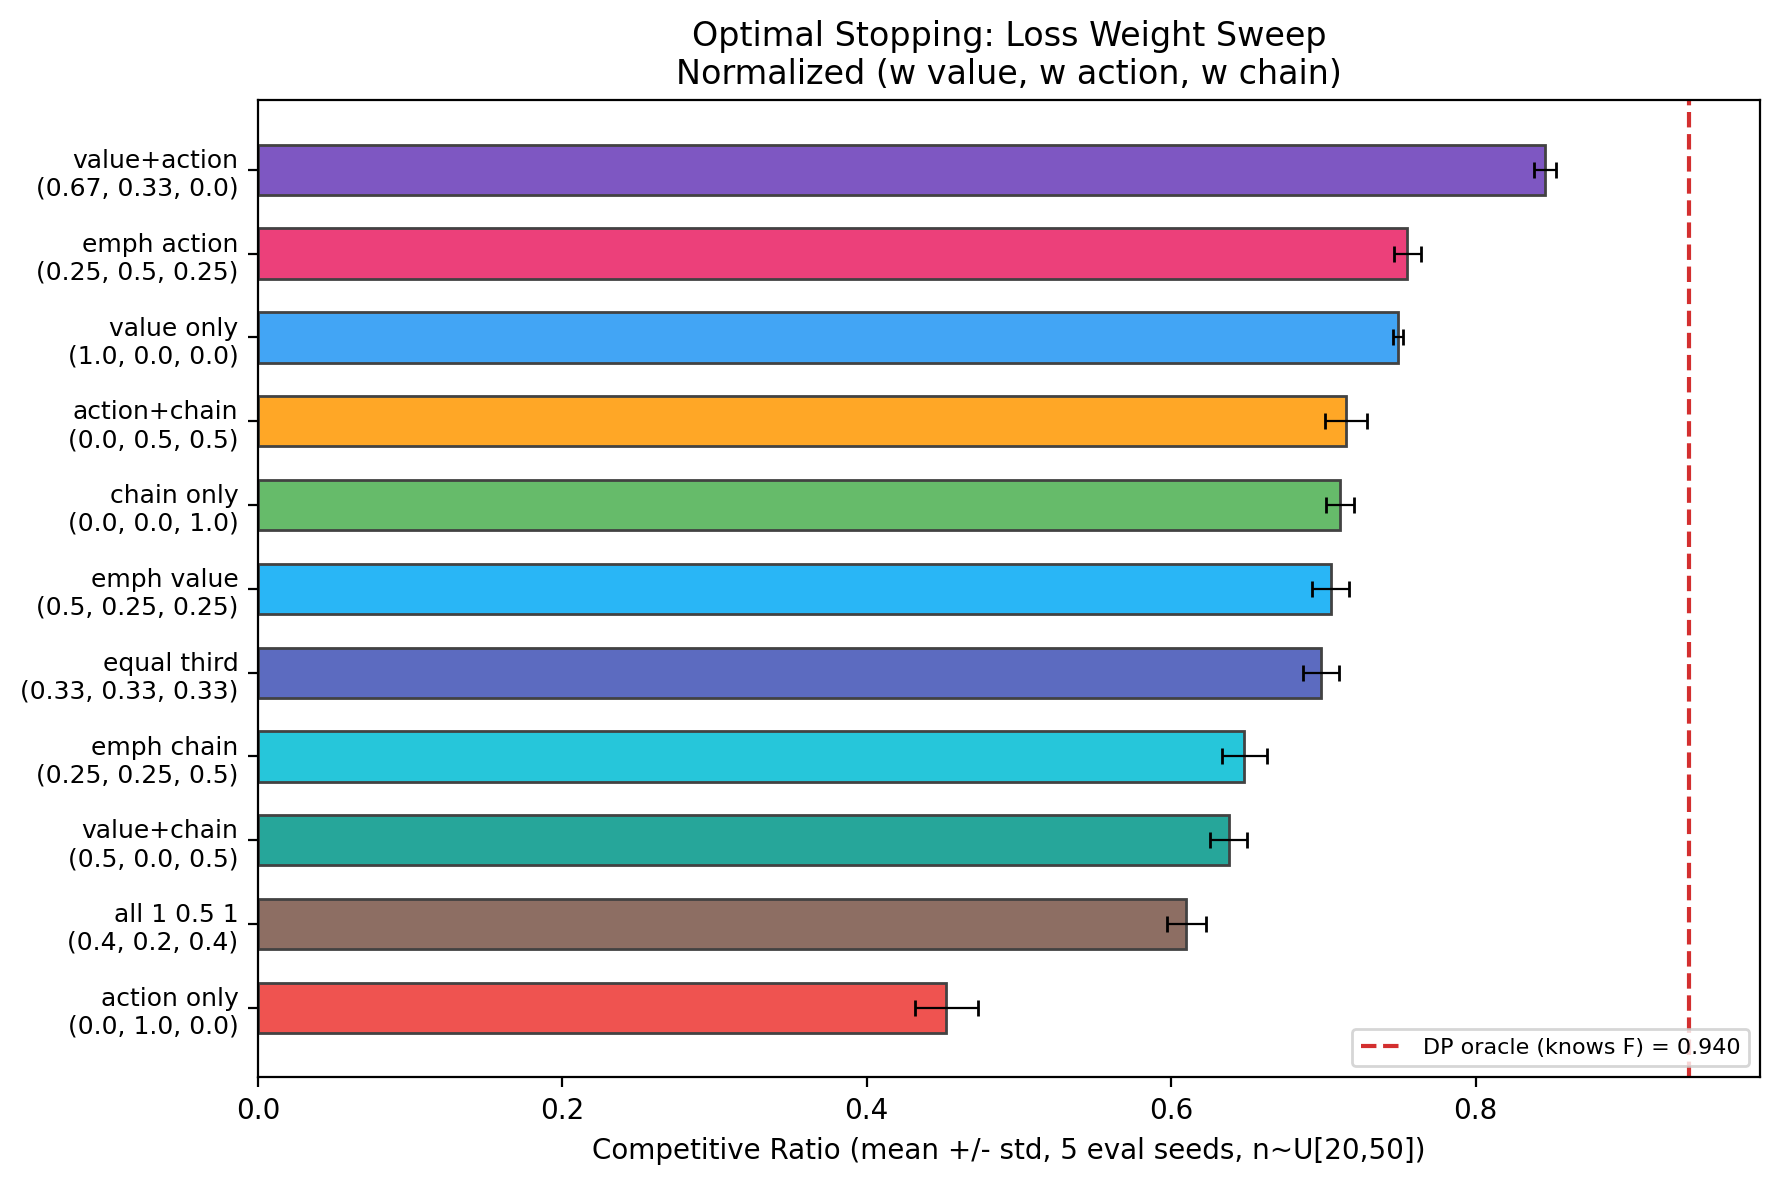
\includegraphics[width=0.85\linewidth]{plots/exp1_loss_weights/ranking_stopping.png}
\caption{Exp~1: Configs ranked by CR. DP oracle dashed.}
\end{figure}

\begin{figure}[h]
\centering
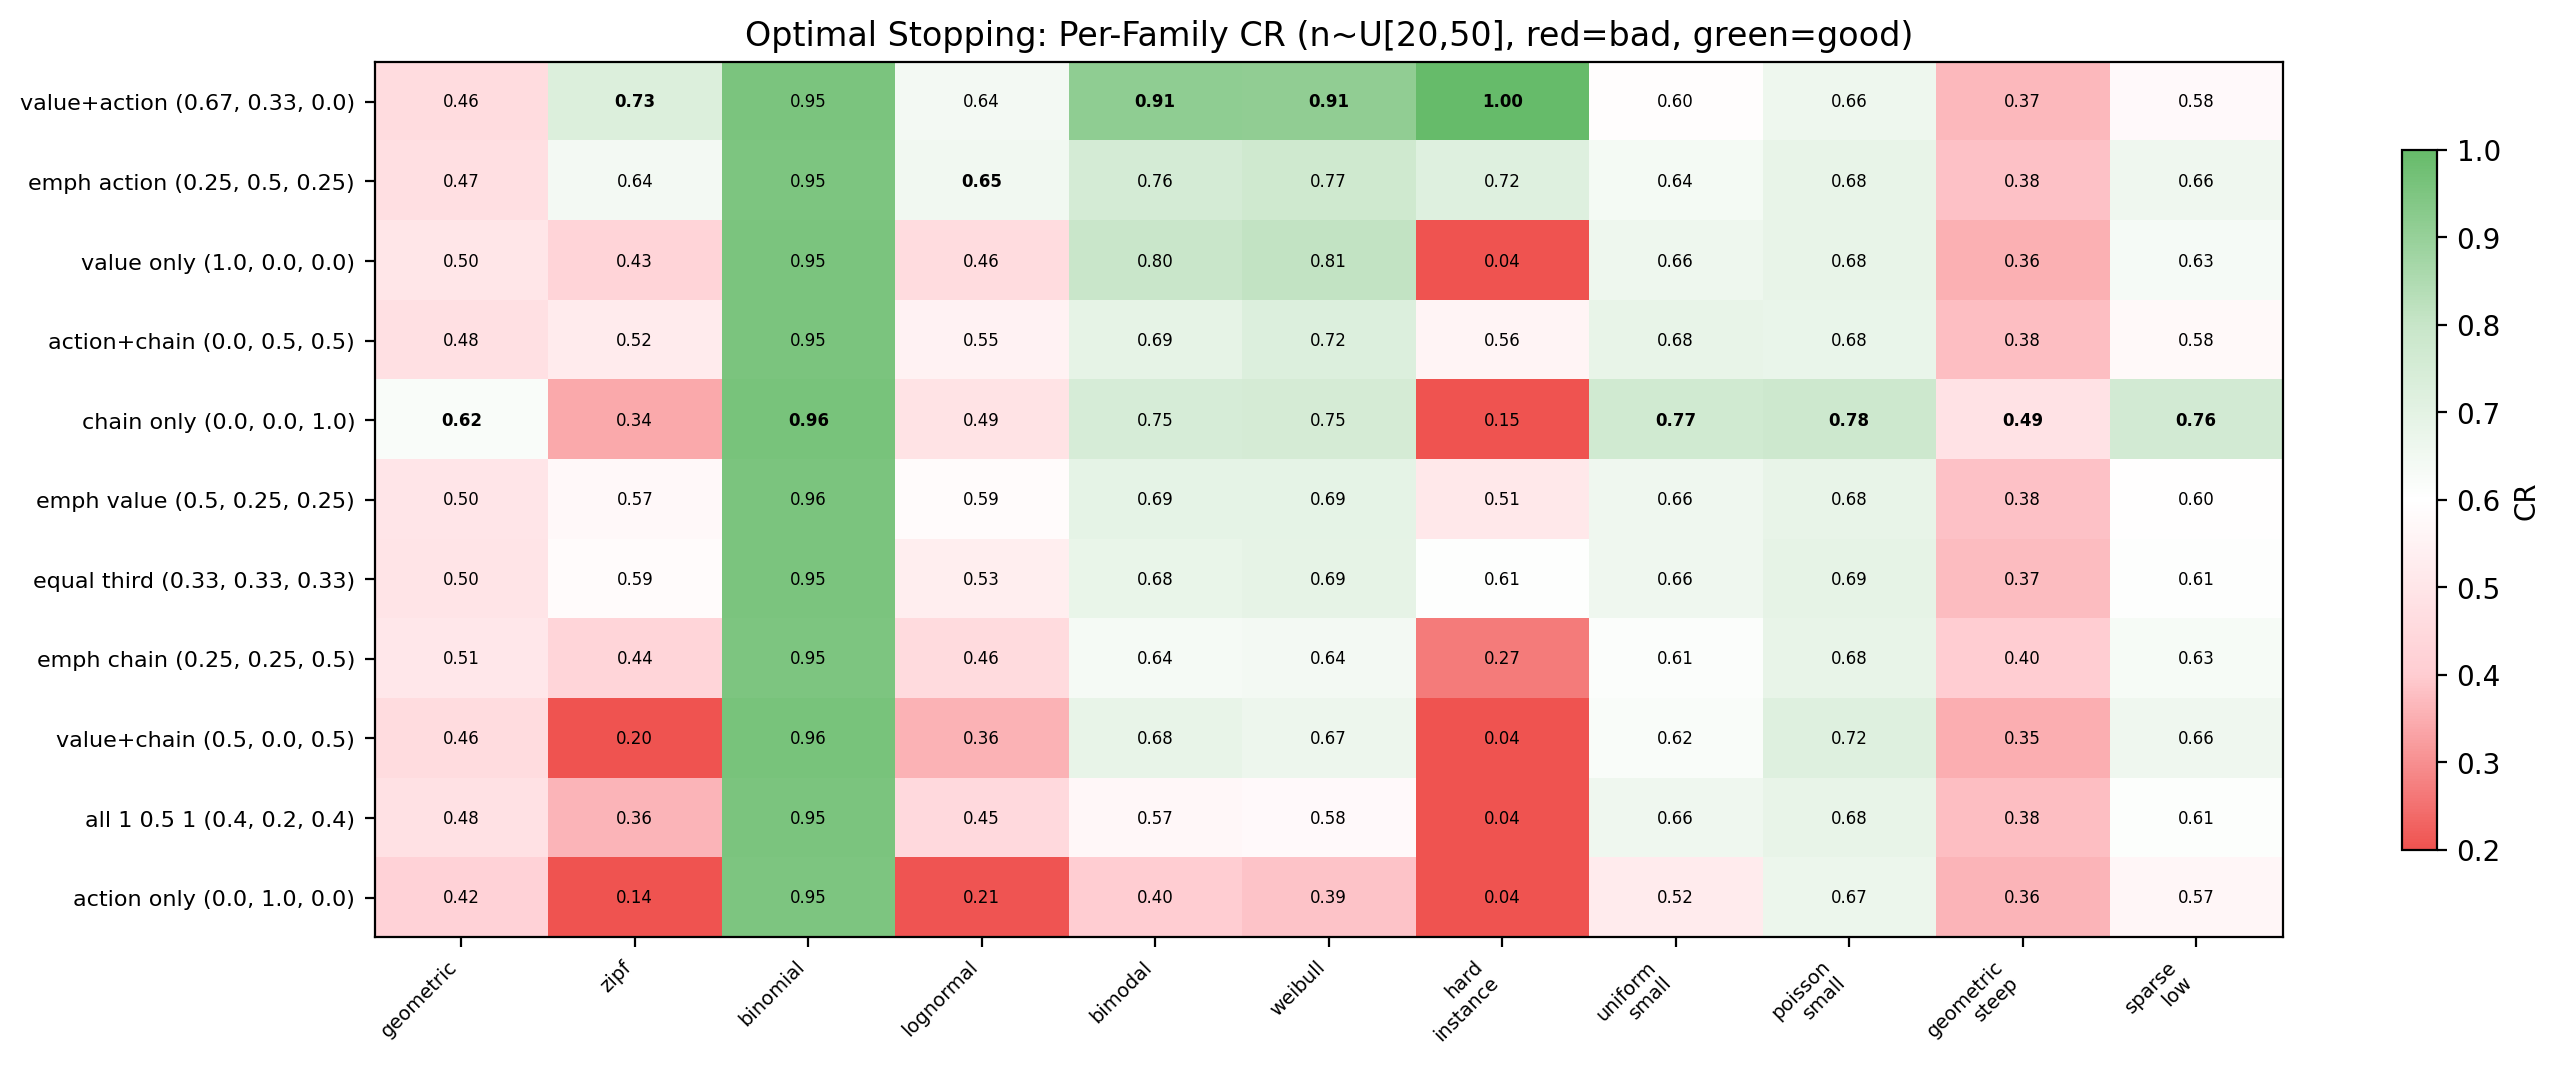
\includegraphics[width=0.95\linewidth]{plots/exp1_loss_weights/per_family_cr_stopping.png}
\caption{Exp~1: Per-family CR across 11 distribution families (red=low, green=high).}
\end{figure}

\begin{figure}[h]
\centering
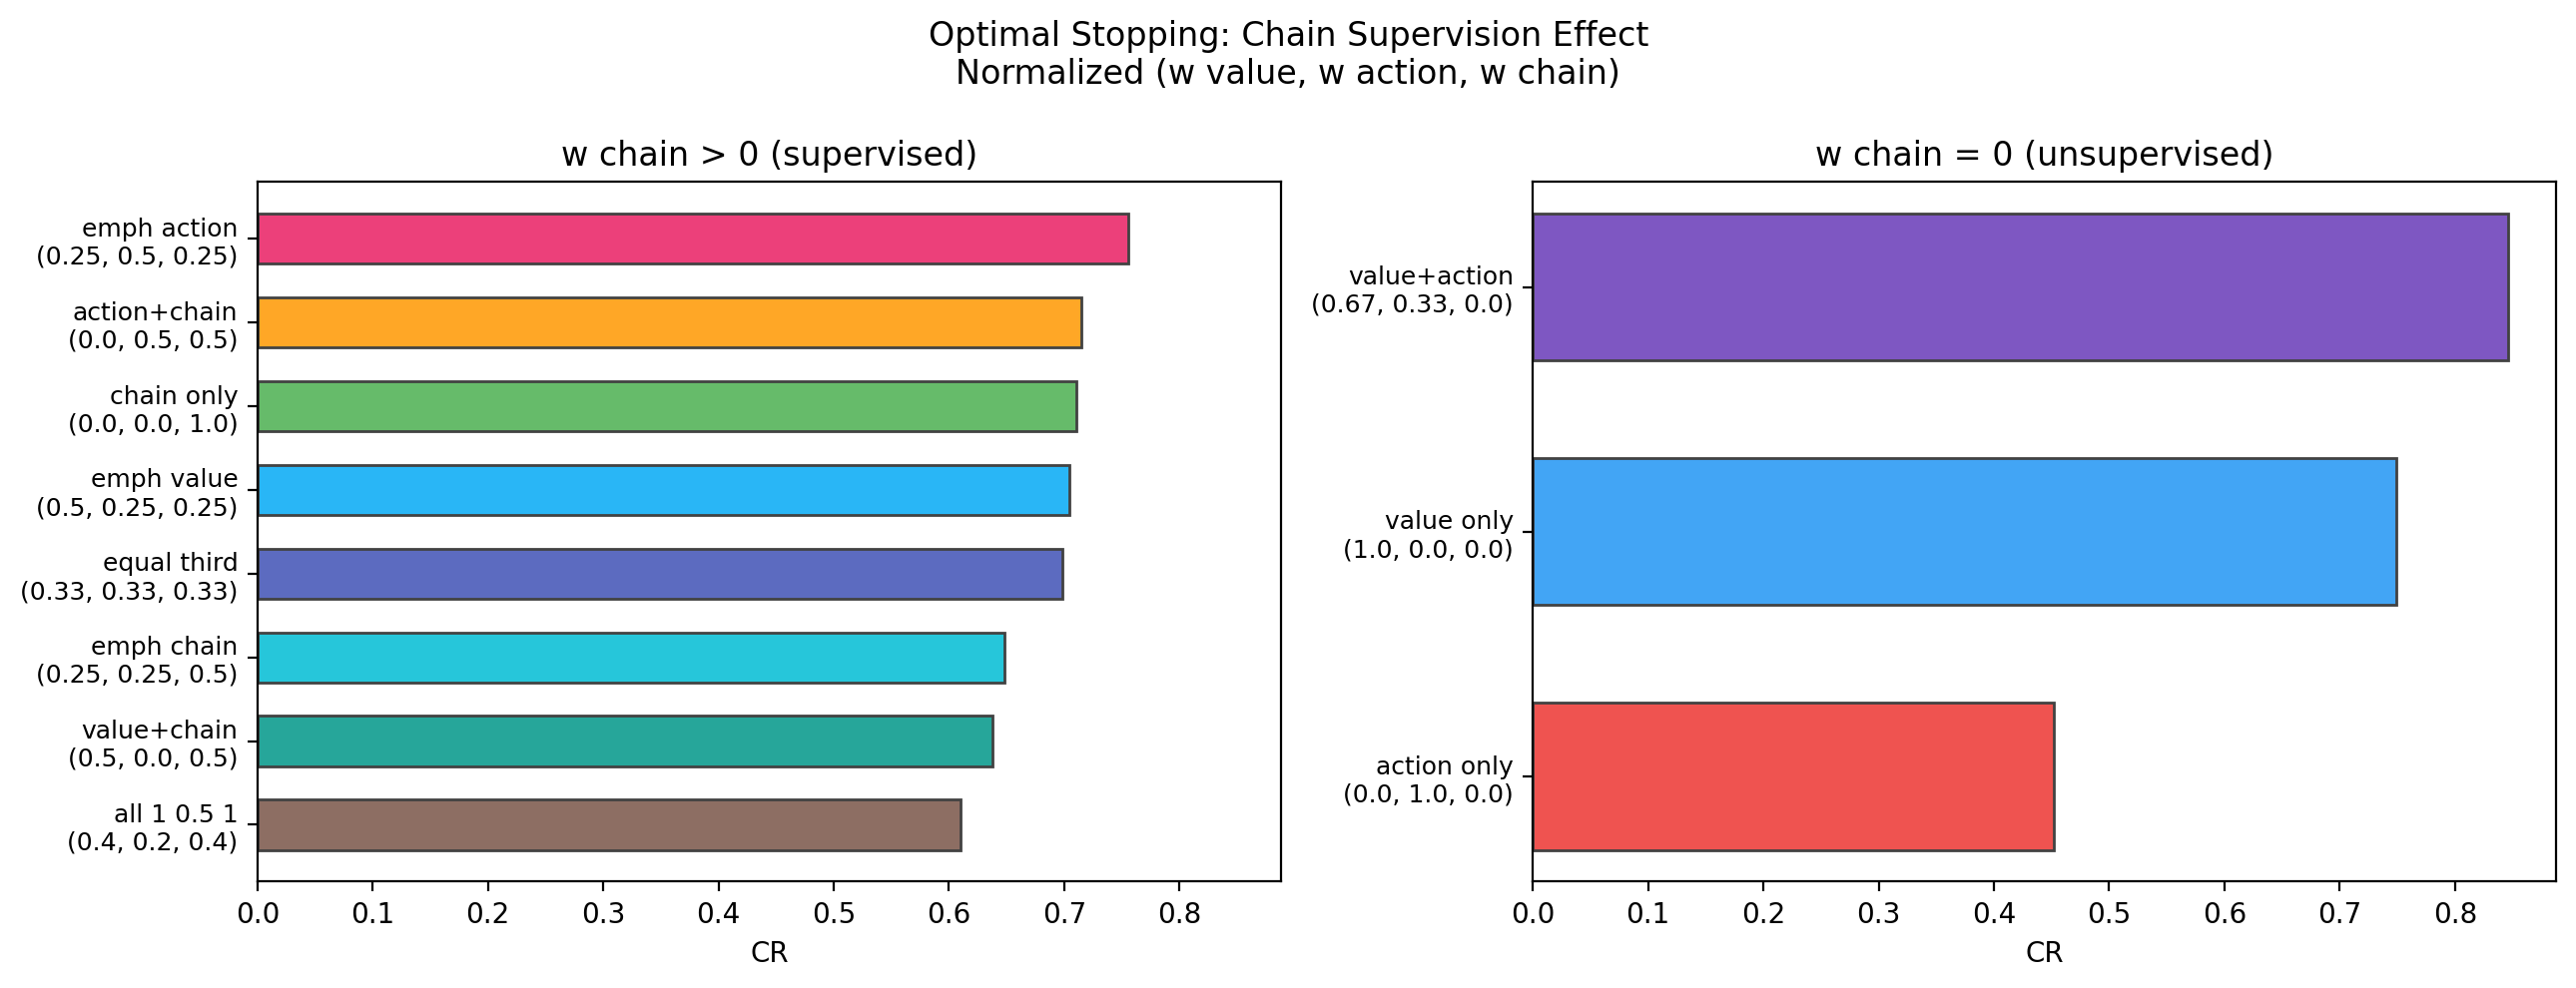
\includegraphics[width=0.85\linewidth]{plots/exp1_loss_weights/chain_effect_stopping.png}
\caption{Exp~1: Chain supervision effect. Left: $w_c > 0$. Right: $w_c = 0$.}
\end{figure}

\begin{figure}[h]
\centering
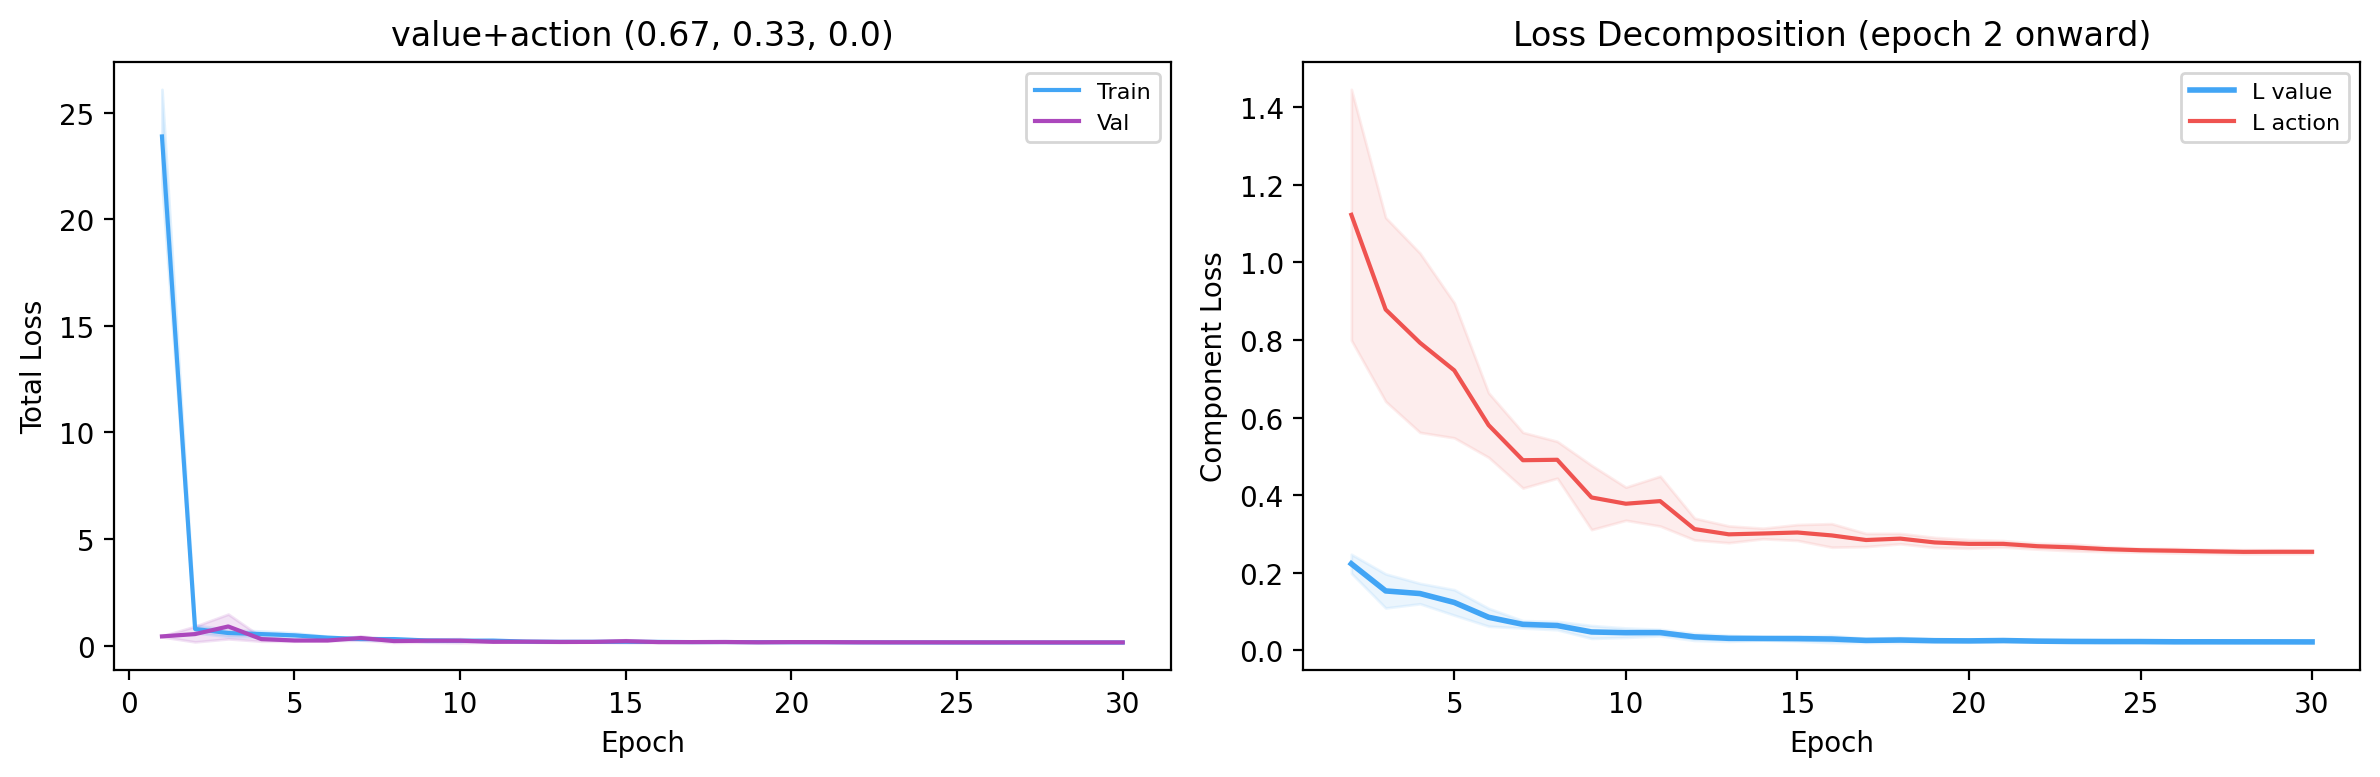
\includegraphics[width=0.48\linewidth]{plots/exp1_loss_weights/training_curves/training_stopping_value+action.png}
\hfill
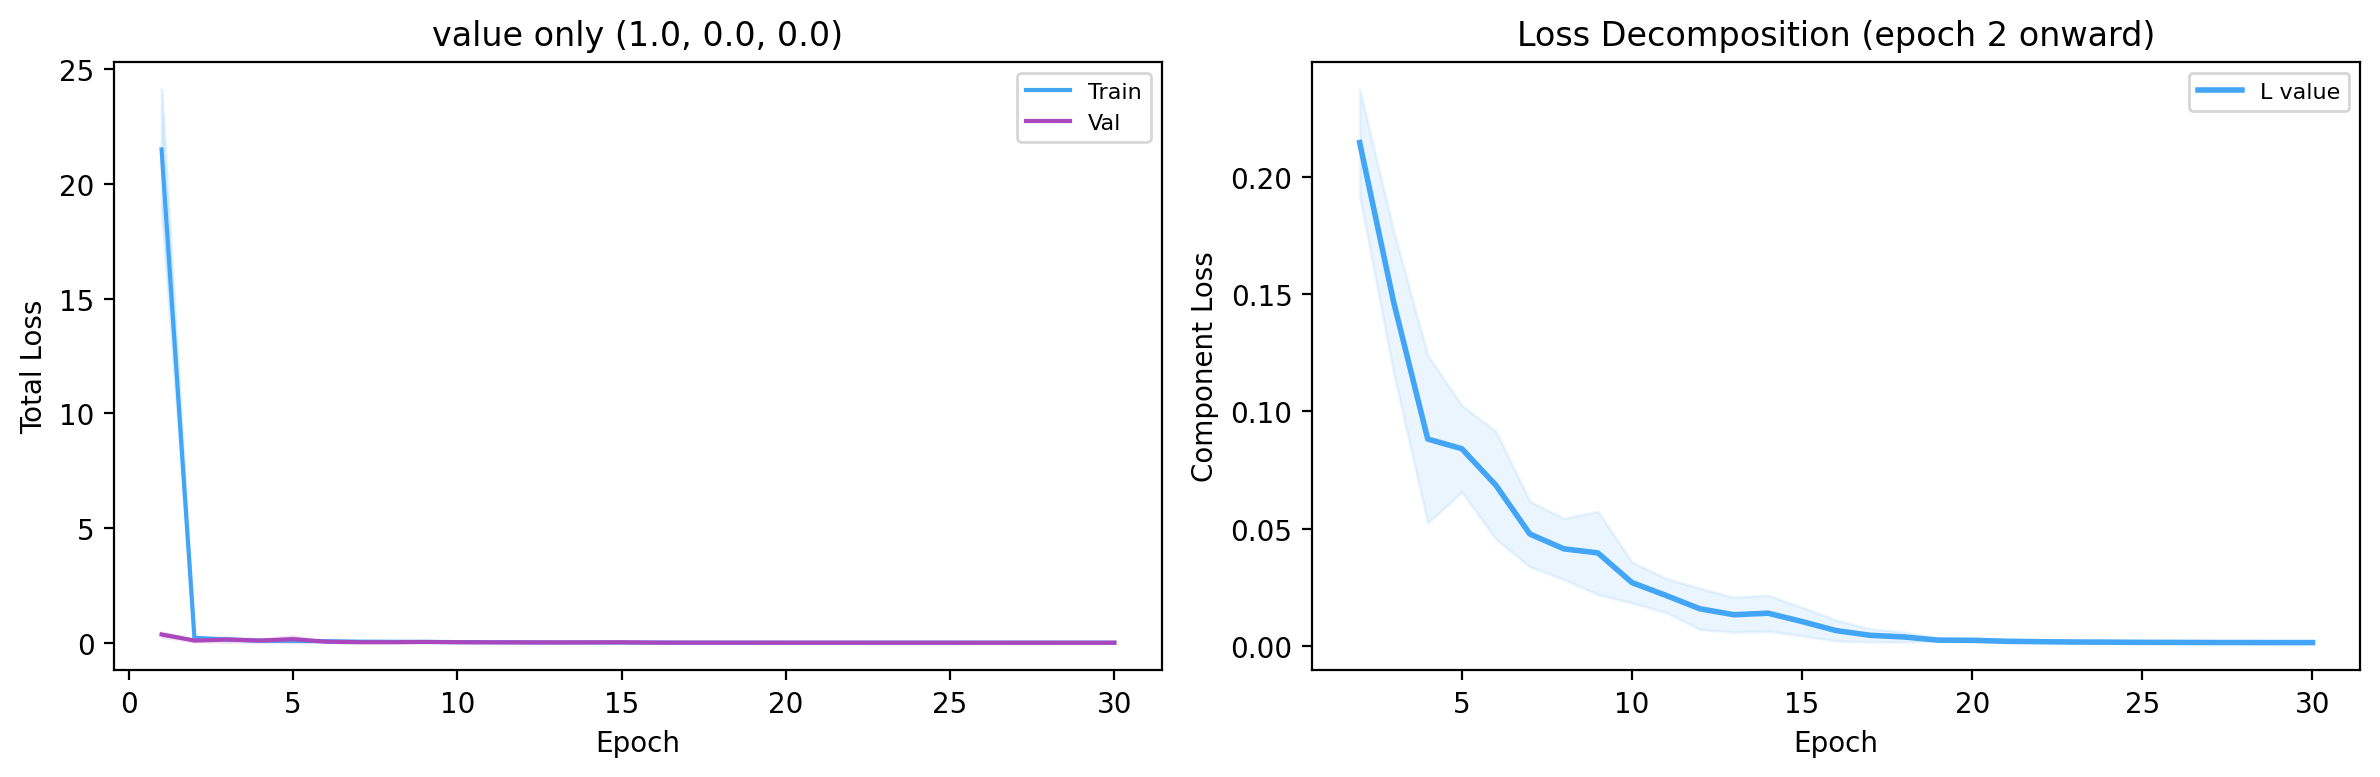
\includegraphics[width=0.48\linewidth]{plots/exp1_loss_weights/training_curves/training_stopping_value_only.png}
\caption{Exp~1: Training curves for value+action (left) vs value only (right). Adding $L_{\mathrm{action}}$ stabilizes training and improves convergence.}
\end{figure}

\begin{figure}[h]
\centering
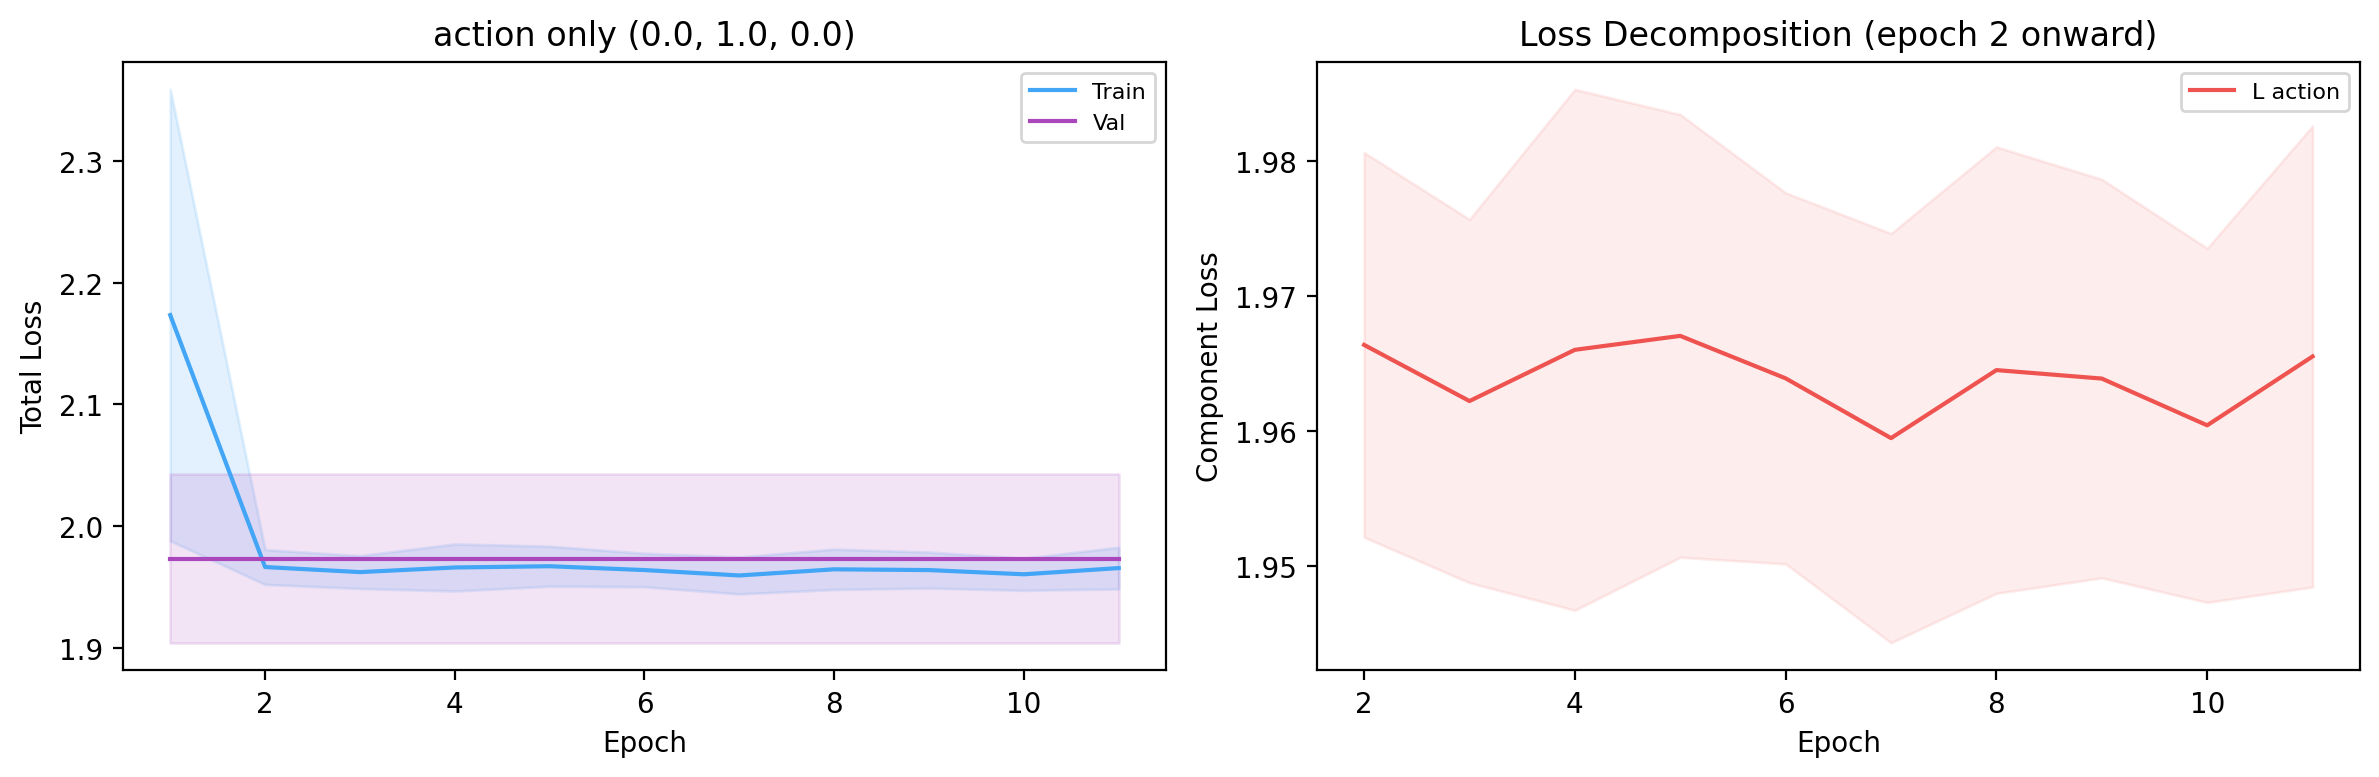
\includegraphics[width=0.48\linewidth]{plots/exp1_loss_weights/training_curves/training_stopping_action_only.png}
\hfill
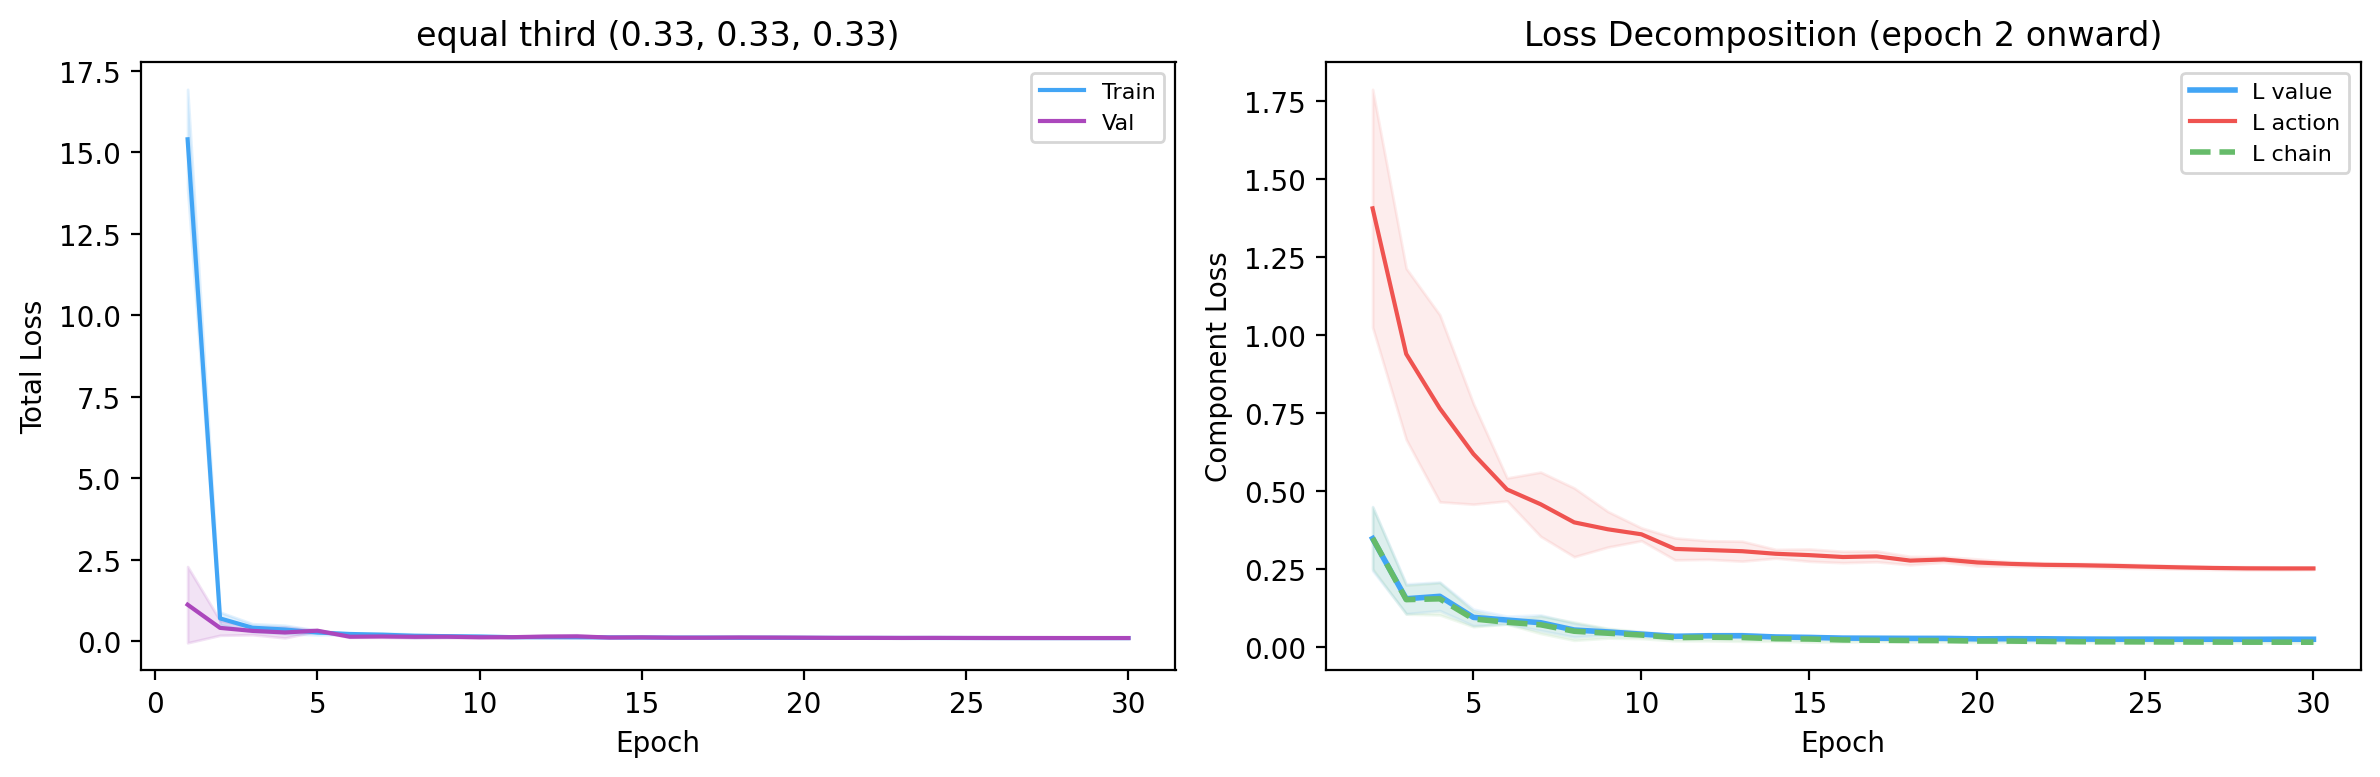
\includegraphics[width=0.48\linewidth]{plots/exp1_loss_weights/training_curves/training_stopping_equal_third.png}
\caption{Exp~1: Action only (left) fails to learn meaningful values. Equal third (right) converges but underperforms value+action.}
\end{figure}

\subsection{Experiment 2: Robust-aware training}

For $\beta \in \{0.05, \ldots, 0.35\}$: masked model (1/3, 1/3, 1/3) vs standard model, both deployed with wrapper.

\begin{figure}[h]
\centering
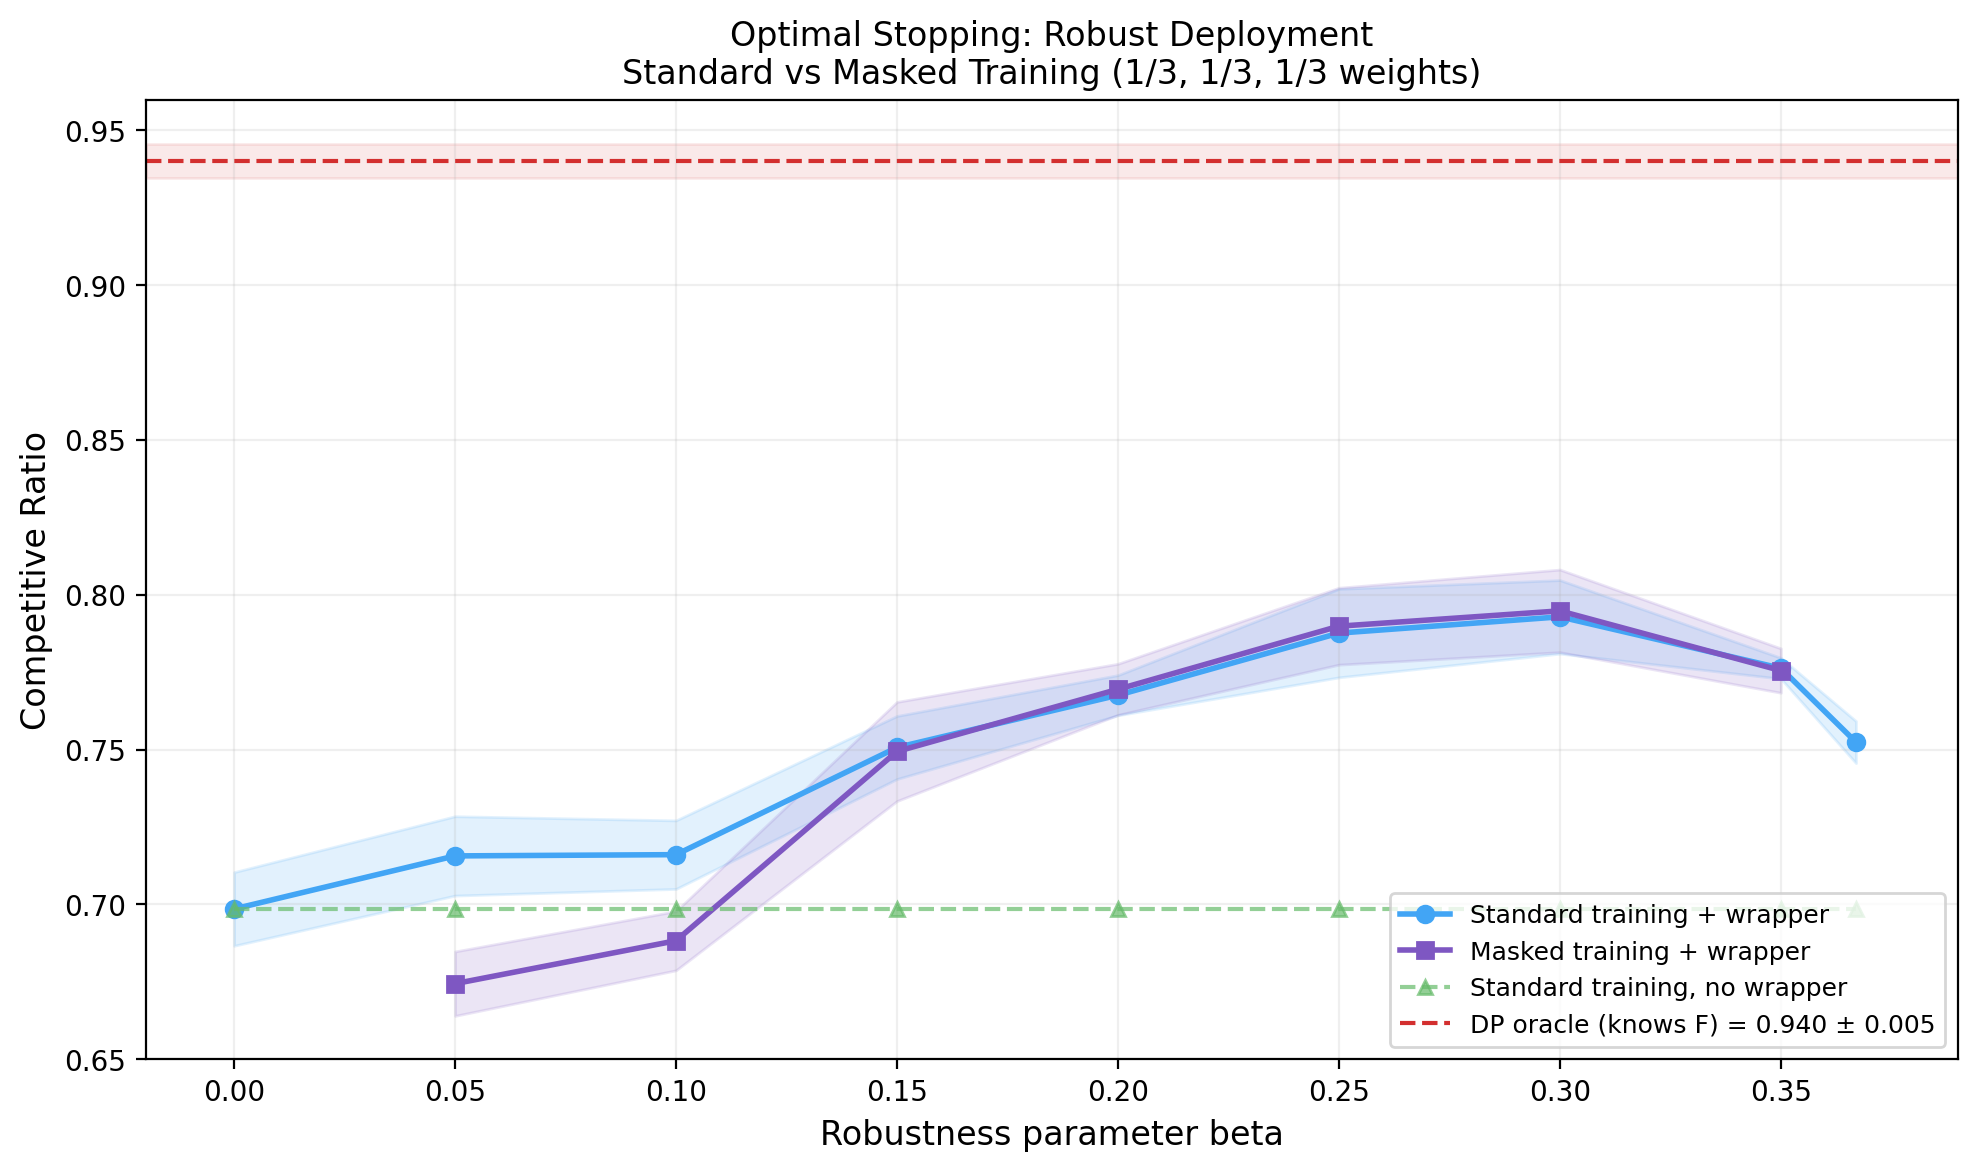
\includegraphics[width=0.85\linewidth]{plots/exp2_robust/robust_cr_vs_beta.png}
\caption{Exp~2: CR vs $\beta$. Standard (blue) and masked (purple) with wrapper, no wrapper (green), DP oracle (red with $\pm$std band).}
\end{figure}

\begin{figure}[h]
\centering
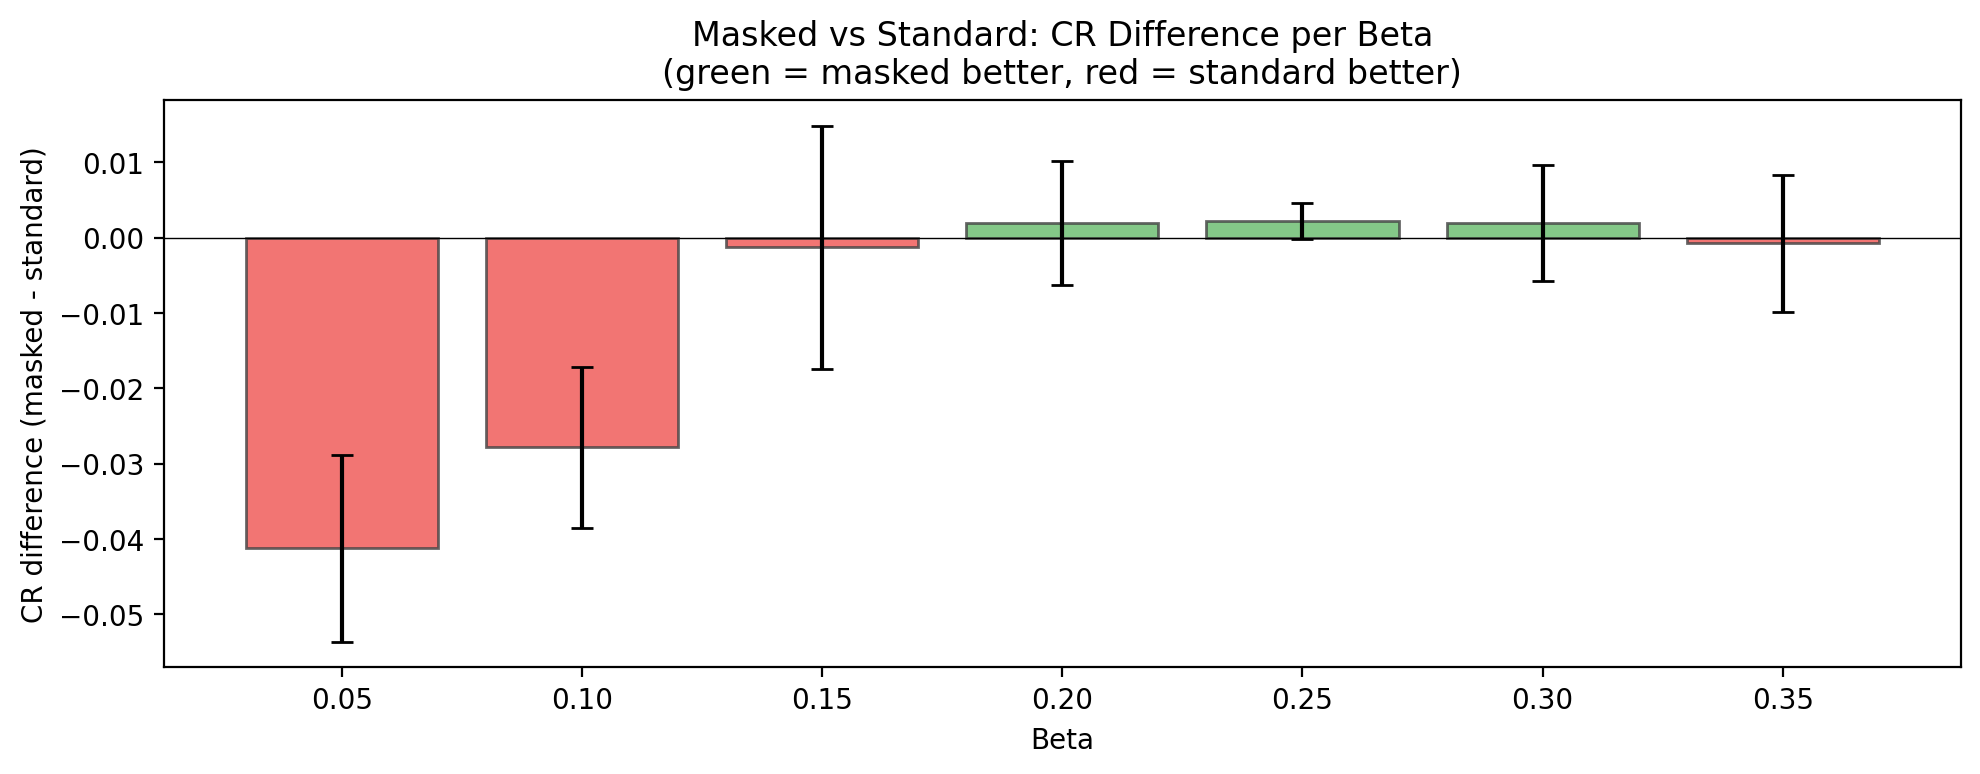
\includegraphics[width=0.85\linewidth]{plots/exp2_robust/robust_cr_diff.png}
\caption{Exp~2: CR difference (masked $-$ standard) per $\beta$. Green=masked better, red=standard better.}
\end{figure}

\begin{figure}[h]
\centering
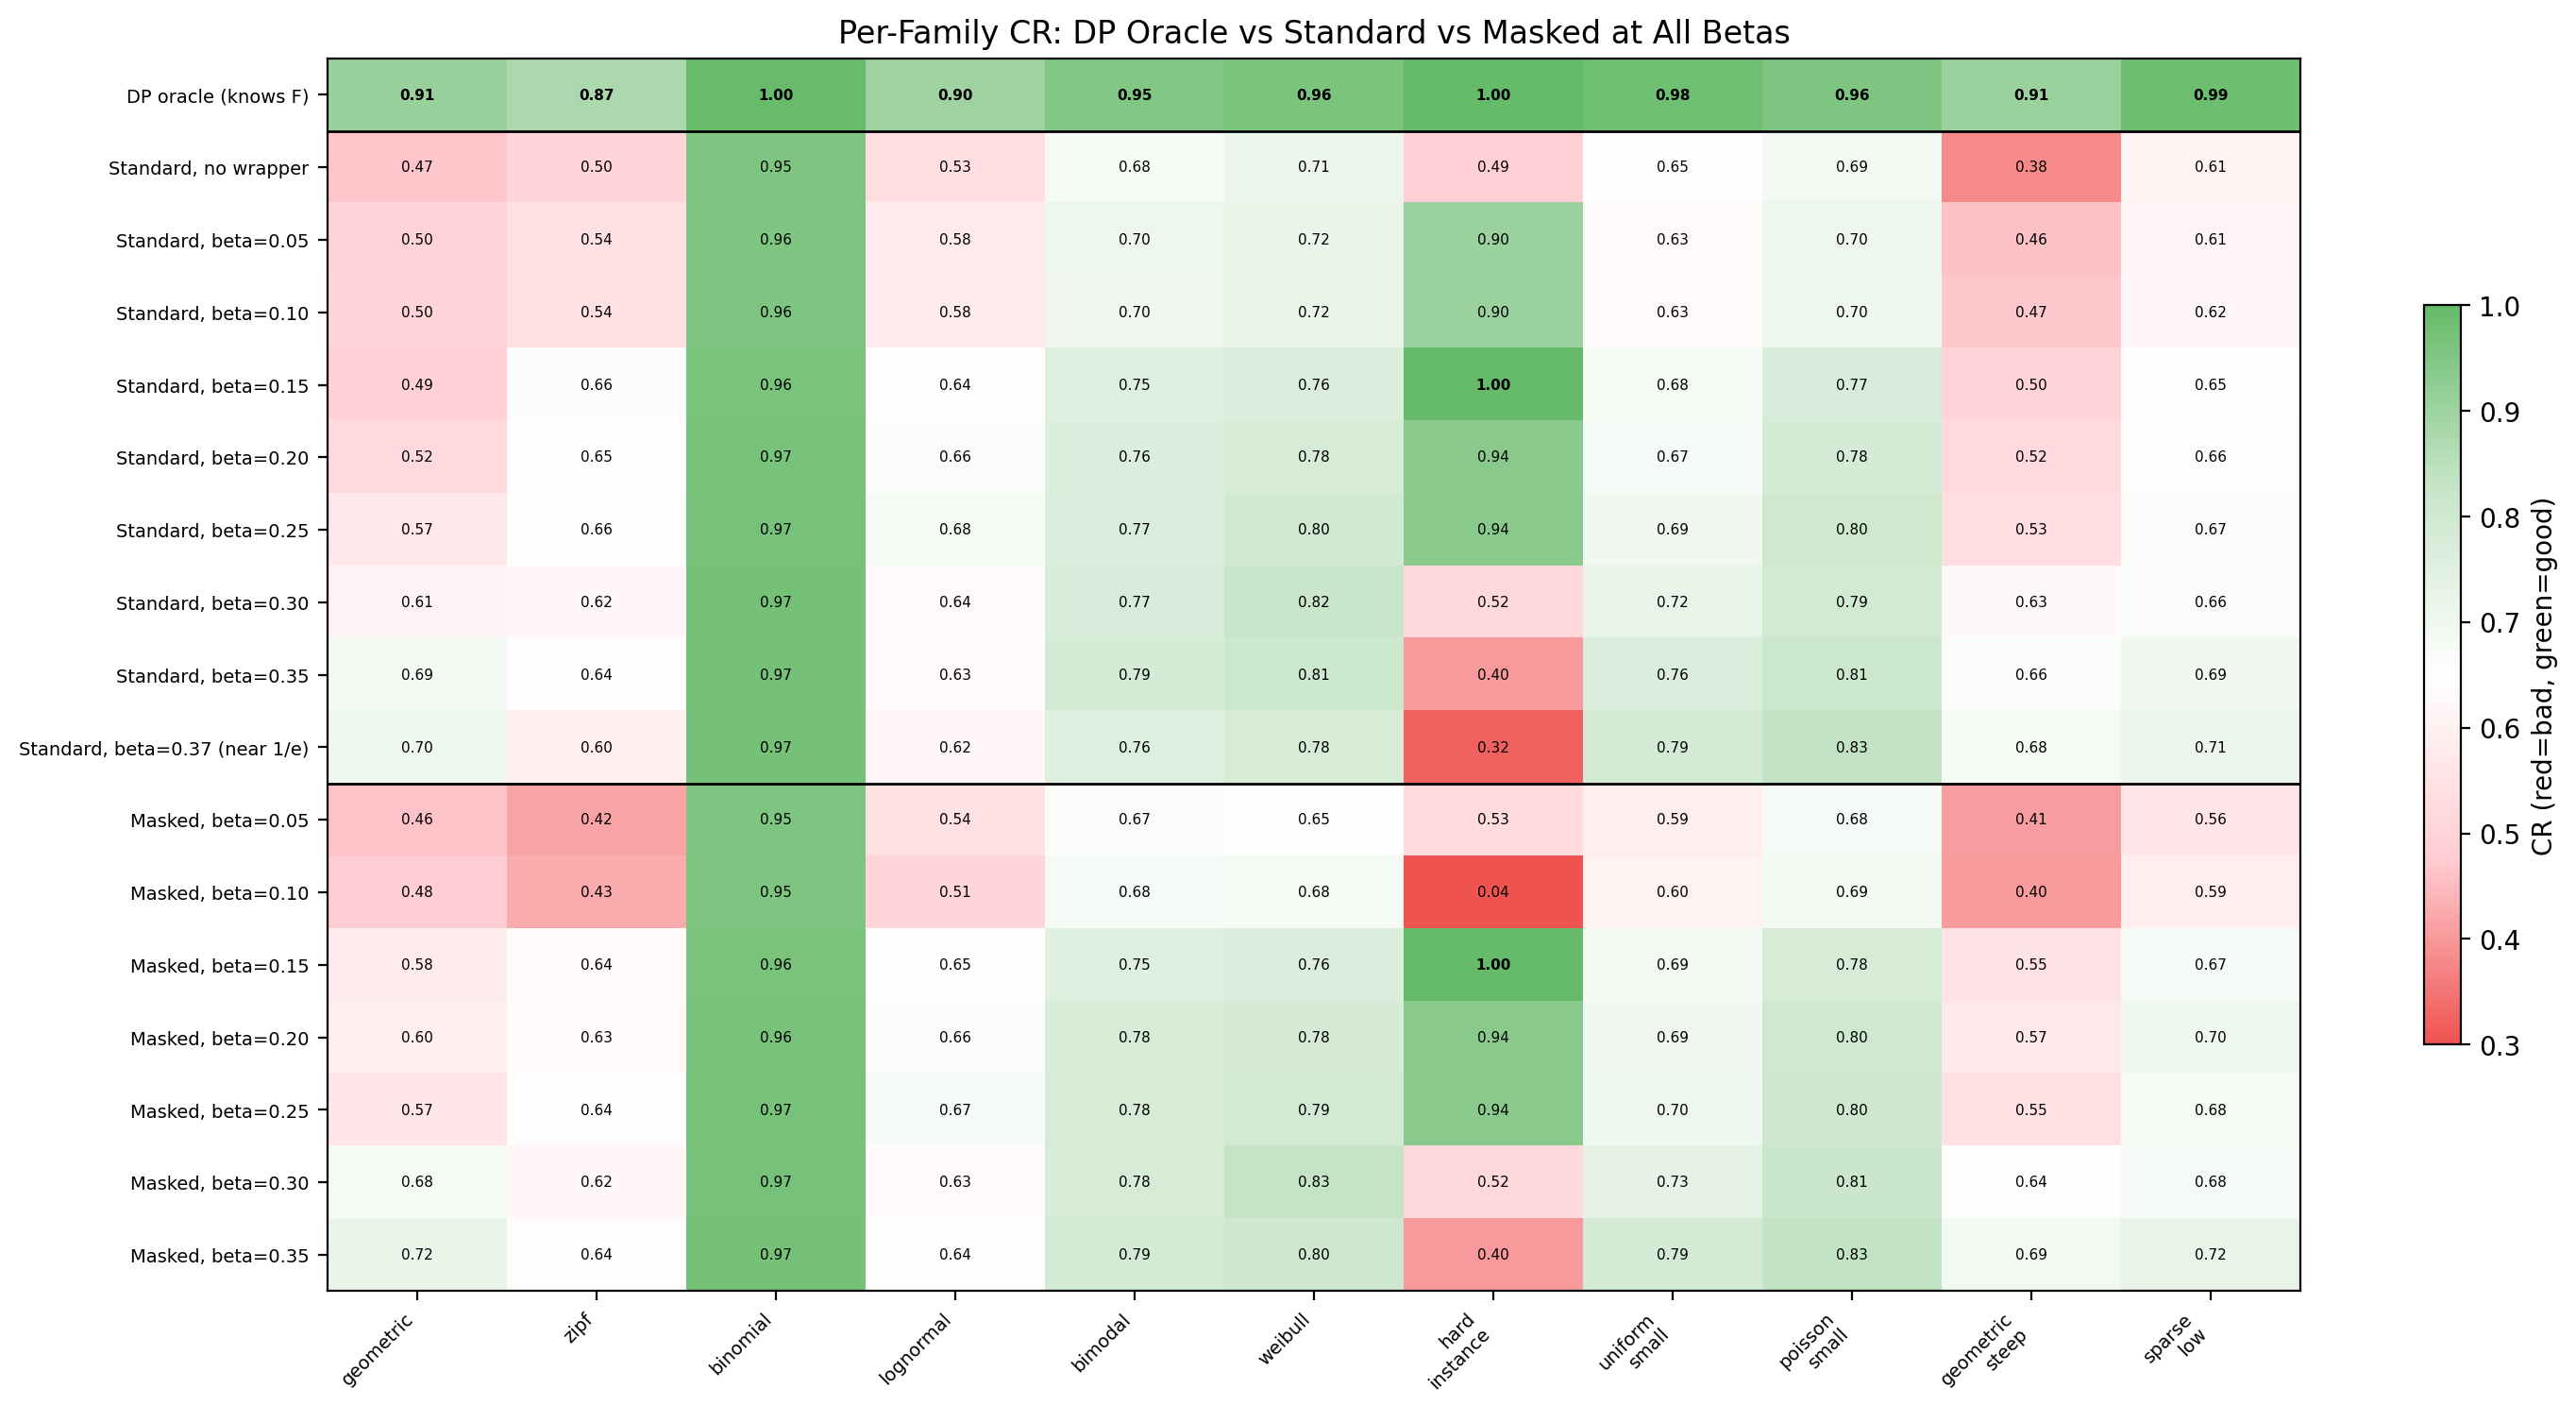
\includegraphics[width=0.95\linewidth]{plots/exp2_robust/robust_per_family_all_betas.png}
\caption{Exp~2: Per-family CR for DP oracle, standard, and masked at all $\beta$.}
\end{figure}

\begin{figure}[h]
\centering
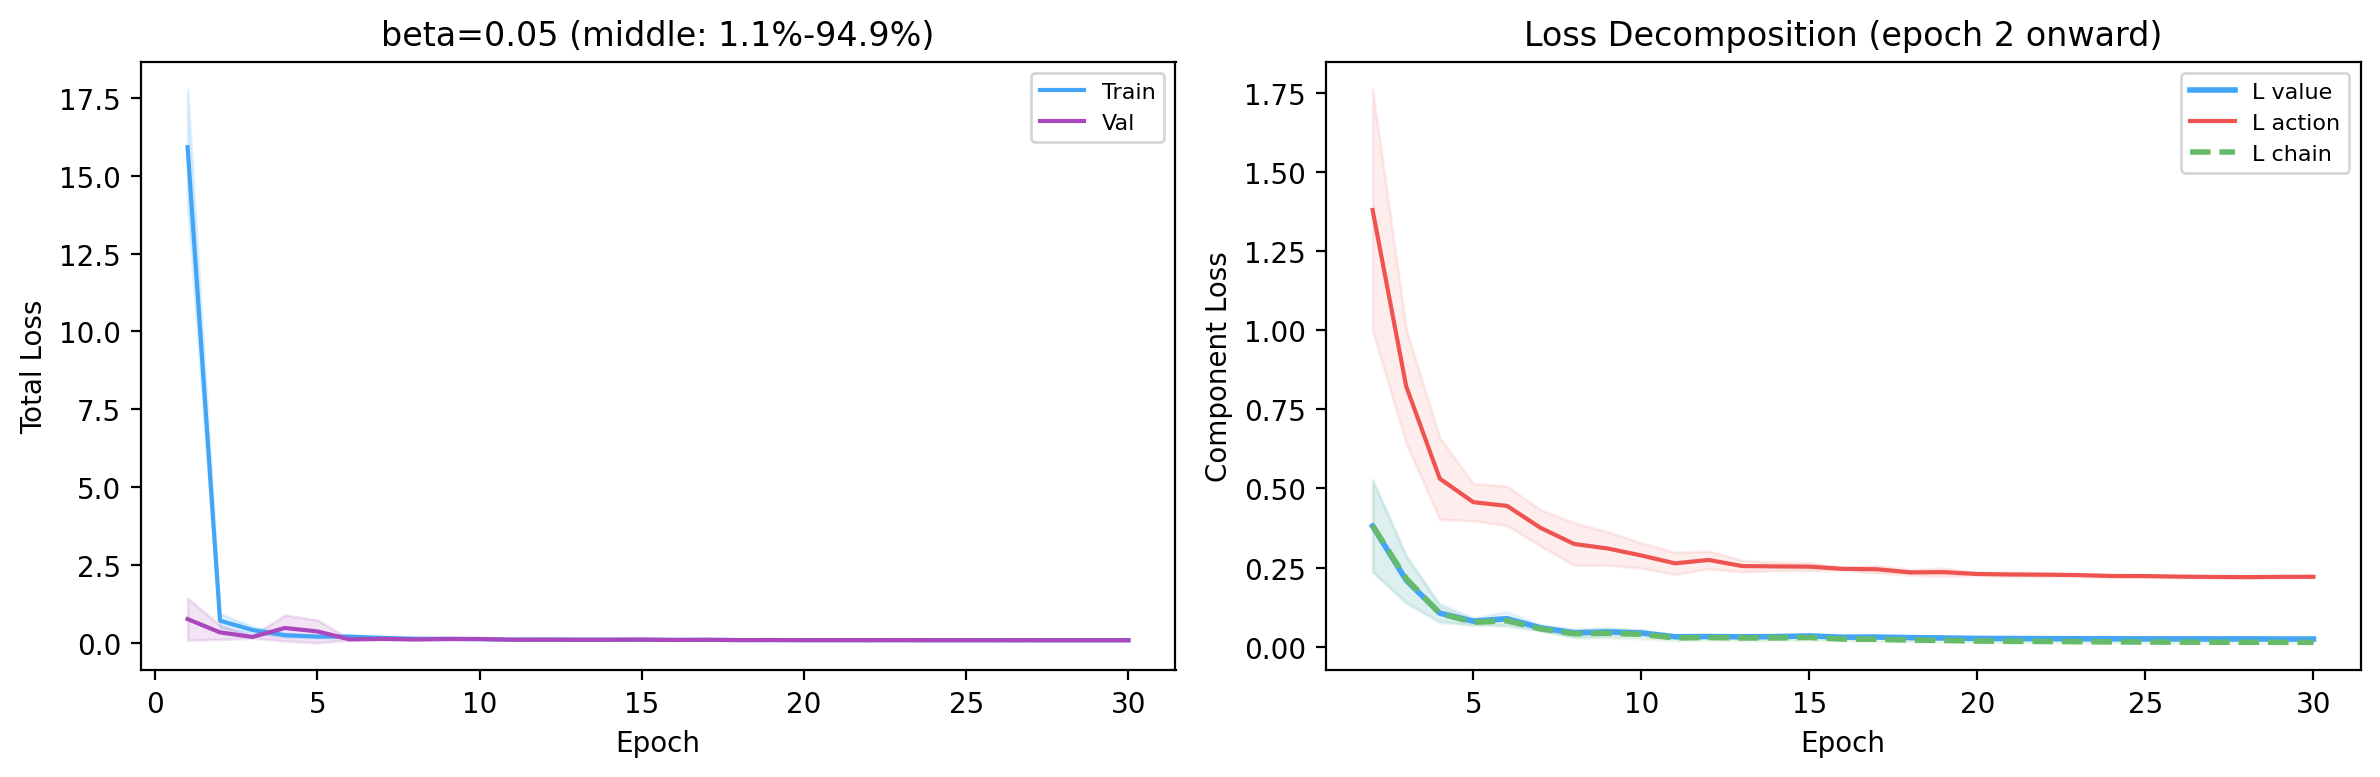
\includegraphics[width=0.48\linewidth]{plots/exp2_robust/robust_training_curves/training_beta0.05.png}
\hfill
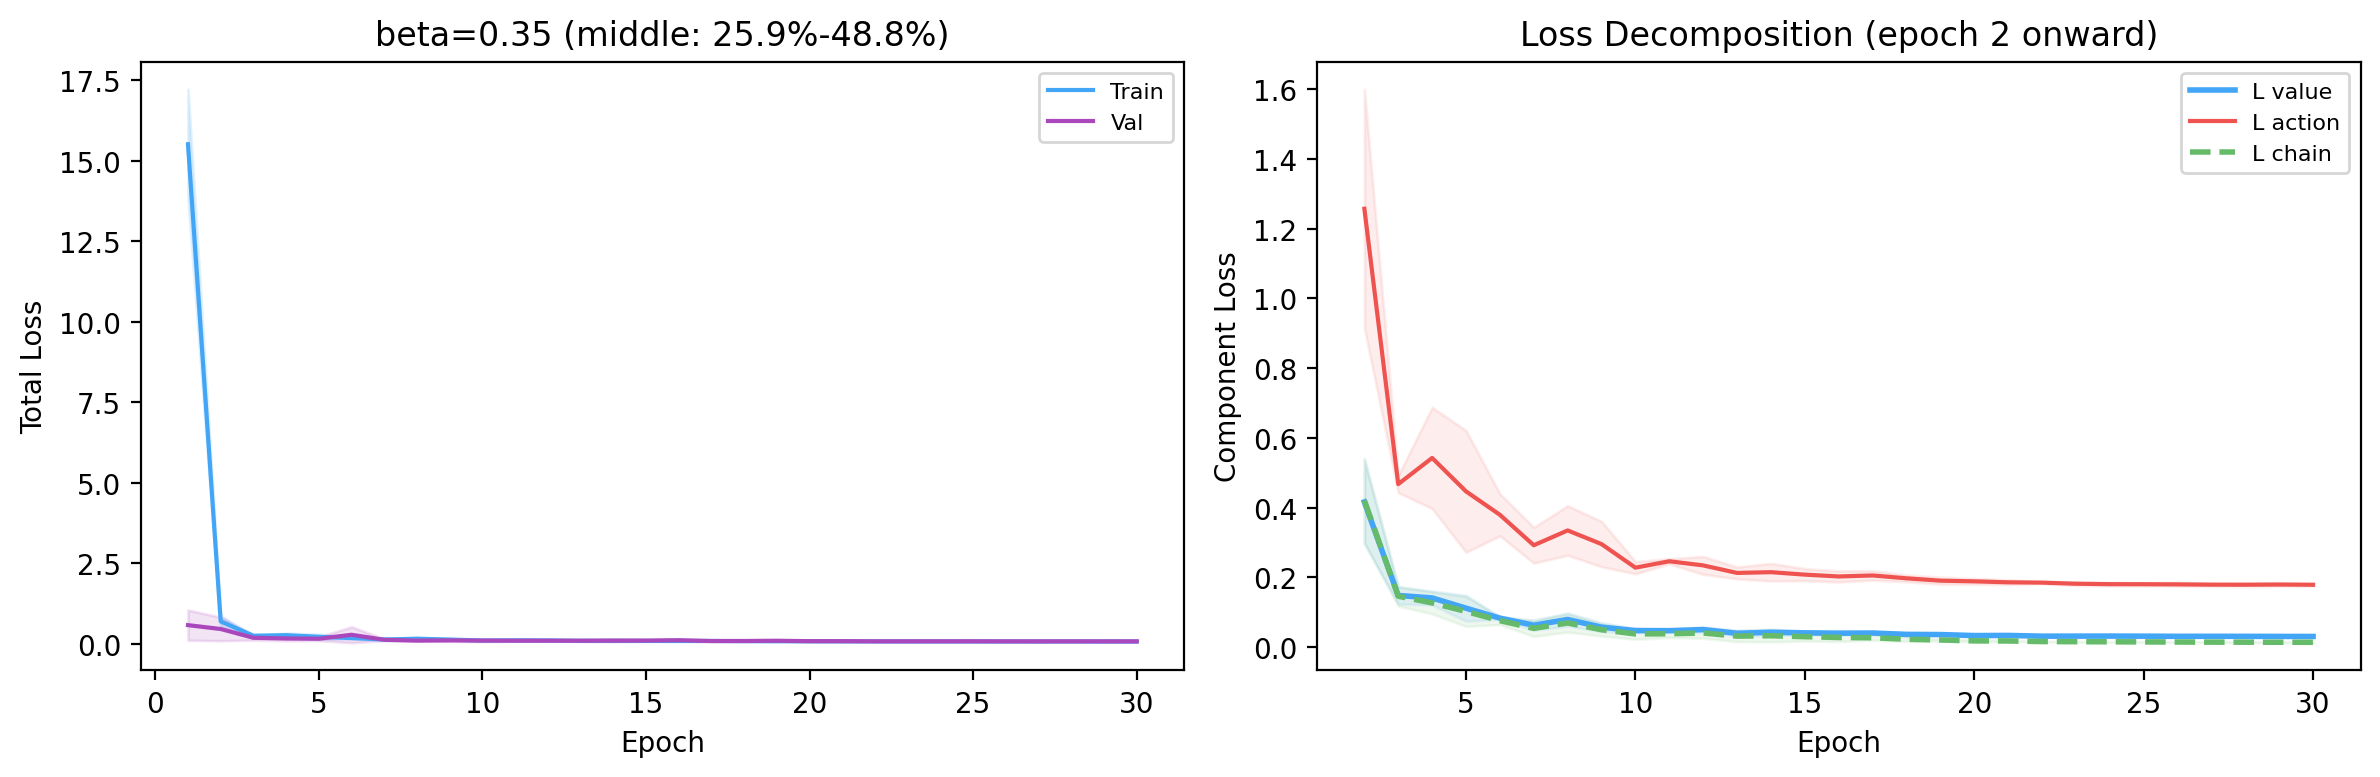
\includegraphics[width=0.48\linewidth]{plots/exp2_robust/robust_training_curves/training_beta0.35.png}
\caption{Exp~2: Training curves for $\beta=0.05$ (left, minimal masking) and $\beta=0.35$ (right, heavy masking).}
\end{figure}

\subsection{Experiment 3: Horizon generalization}

Evaluate at $n \in \{5, 10, 15, 20, 30, 40, 50, 55, 65, 75, 85, 100\}$ (trained on $[20, 50]$). No retraining.

\begin{figure}[h]
\centering
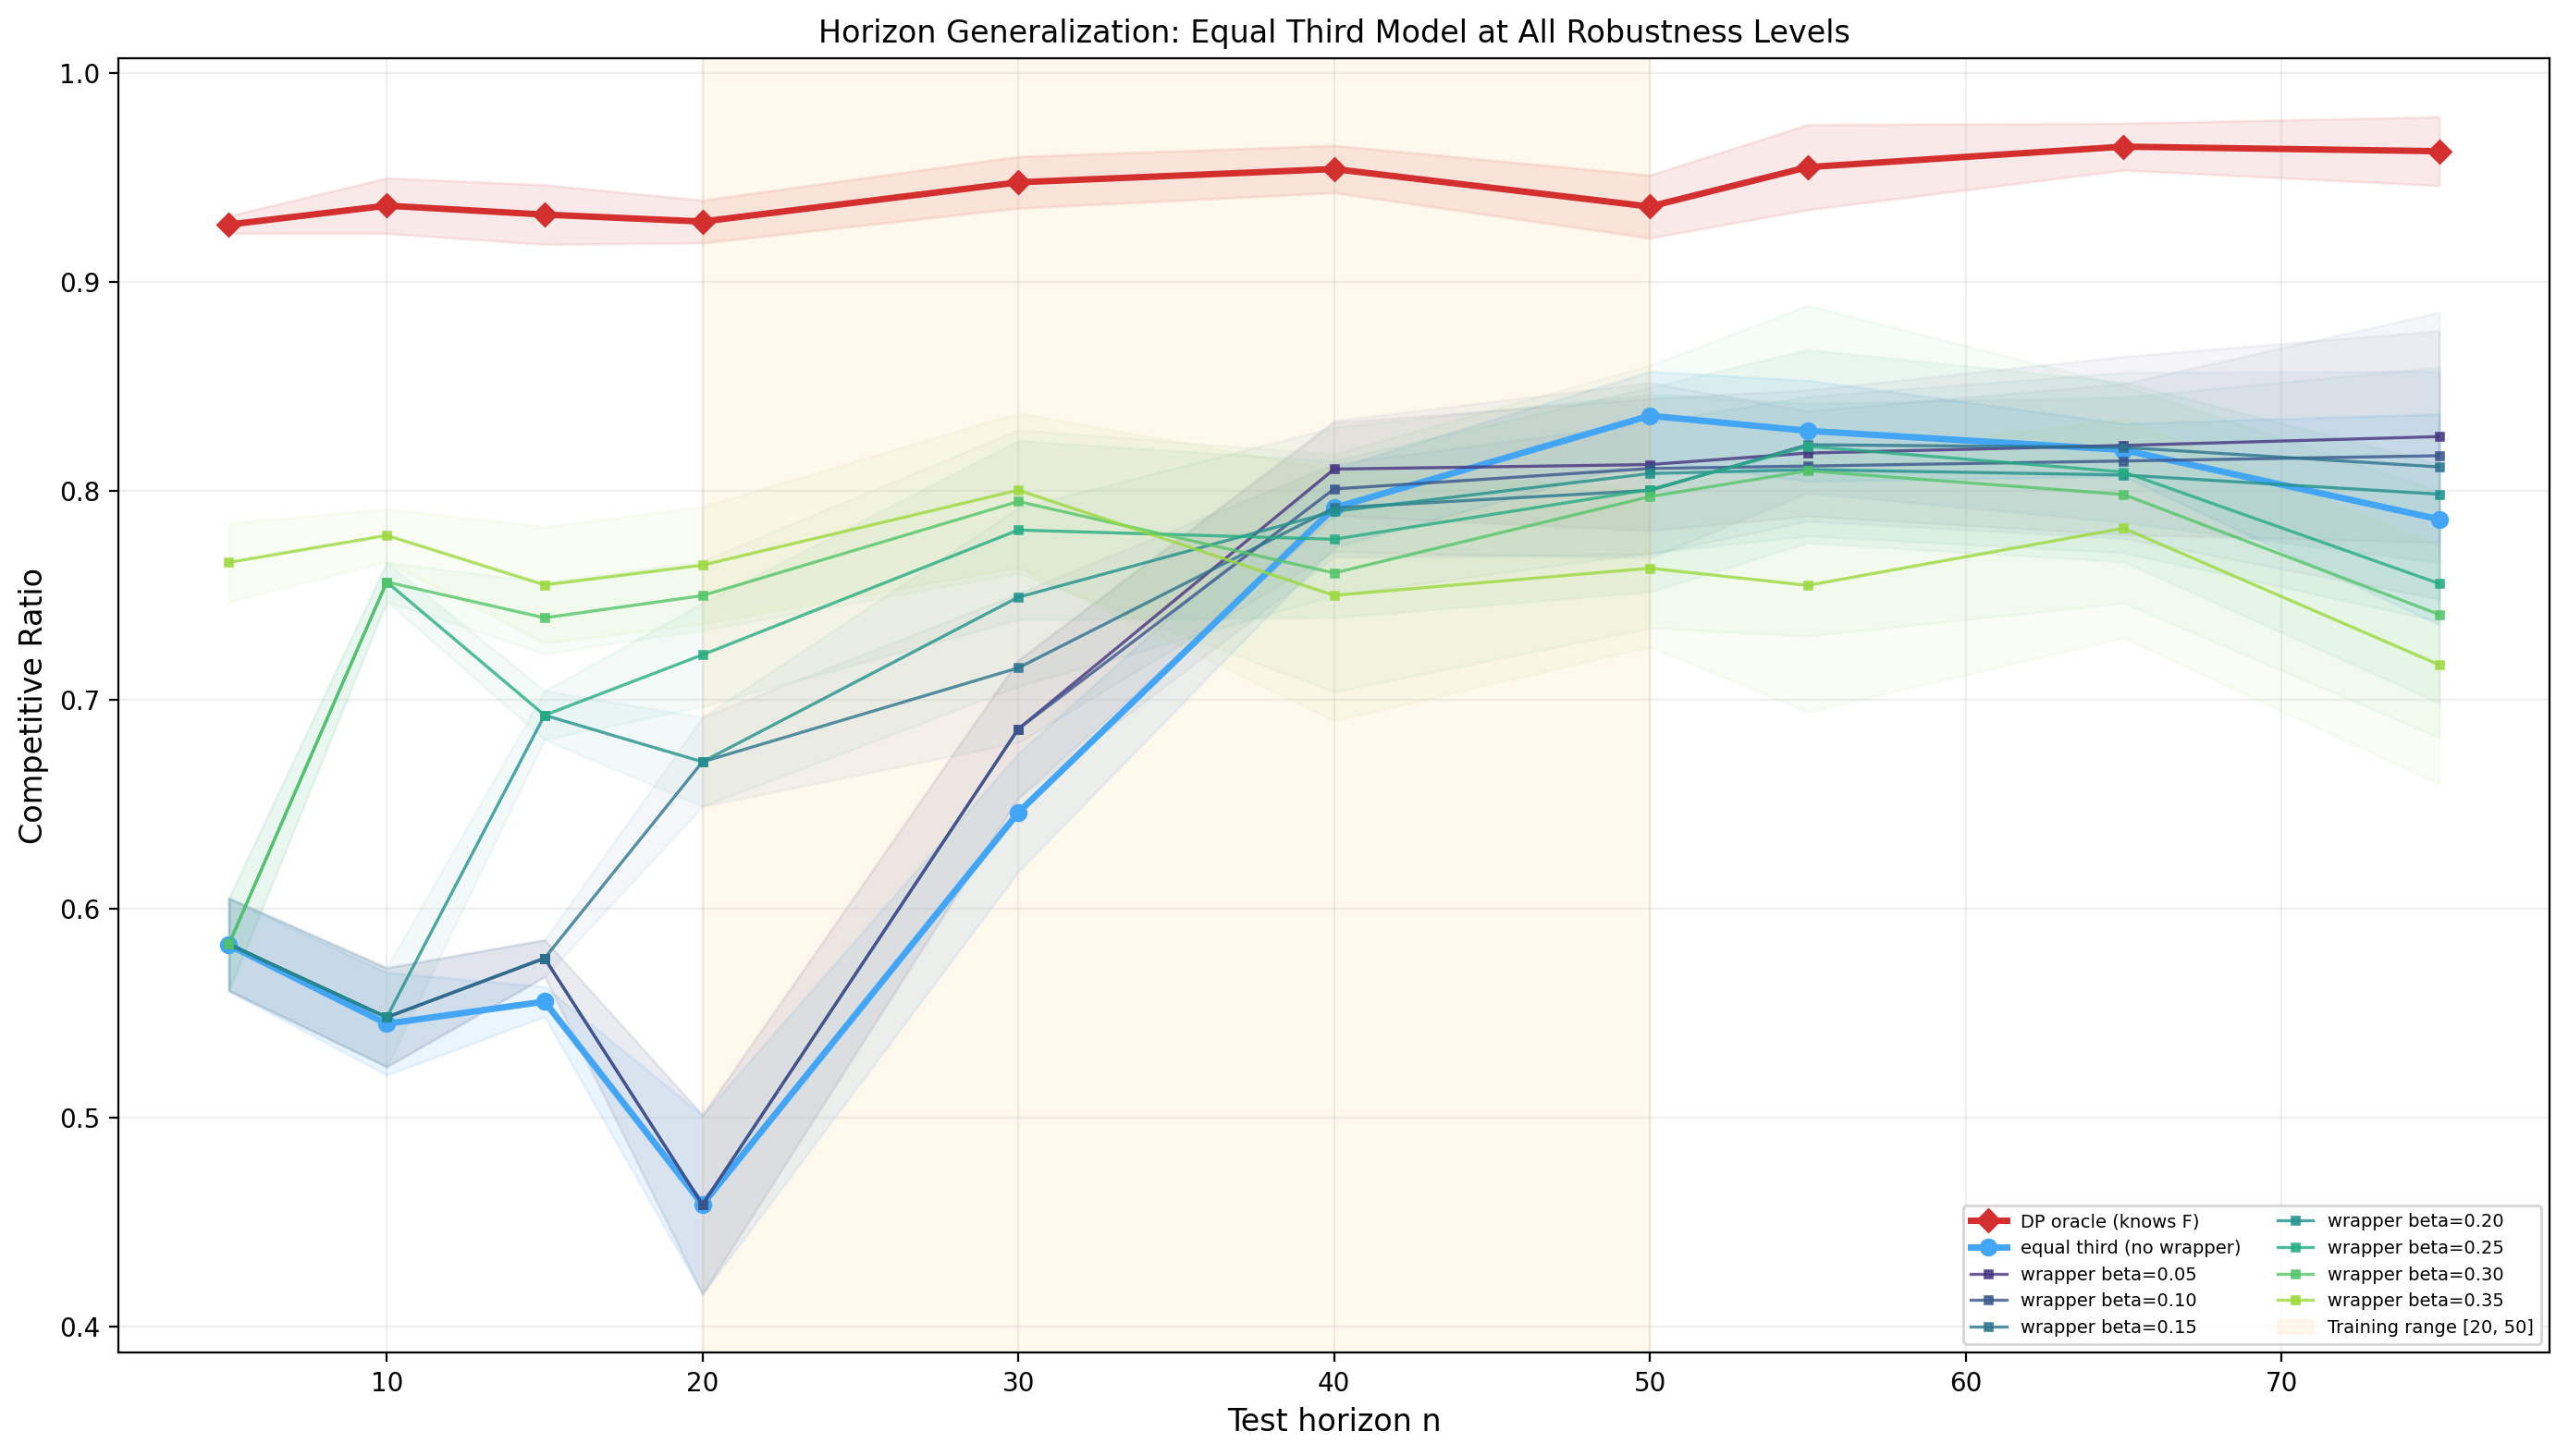
\includegraphics[width=0.85\linewidth]{plots/exp4_horizon/horizon_cr_all_betas.png}
\caption{Exp~3: CR vs test horizon for equal third model at all robustness levels. DP oracle (red), no wrapper (blue), wrapper at each $\beta$ (colored lines). Training range shaded.}
\end{figure}

\subsection{Experiment 4: Attention analysis}

We extract attention weights from the best model (value+action) via teacher-forced forward passes on 5 diverse instances (one per family: geometric, Zipf, binomial, log-normal, bimodal). The 2-layer, 2-head architecture was chosen to match the Proposition~1 construction. We ask: do the learned attention patterns reflect the theoretical roles?

The full attention matrix divides into four quadrants (Figure~\ref{fig:attn-full}). The chain$\to$chain quadrant (bottom-right) in Layer~0 shows a strong nearest-neighbor diagonal: each $V(t,k)$ attends primarily to $V(t,k{+}1)$, consistent with the backward-induction recurrence $C_k = f(C_{k+1})$. Layer~1's chain$\to$observation quadrant (bottom-left) shows diffuse attention across visible observations, consistent with PMF estimation from i.i.d.\ samples.

\begin{figure}[h]
\centering
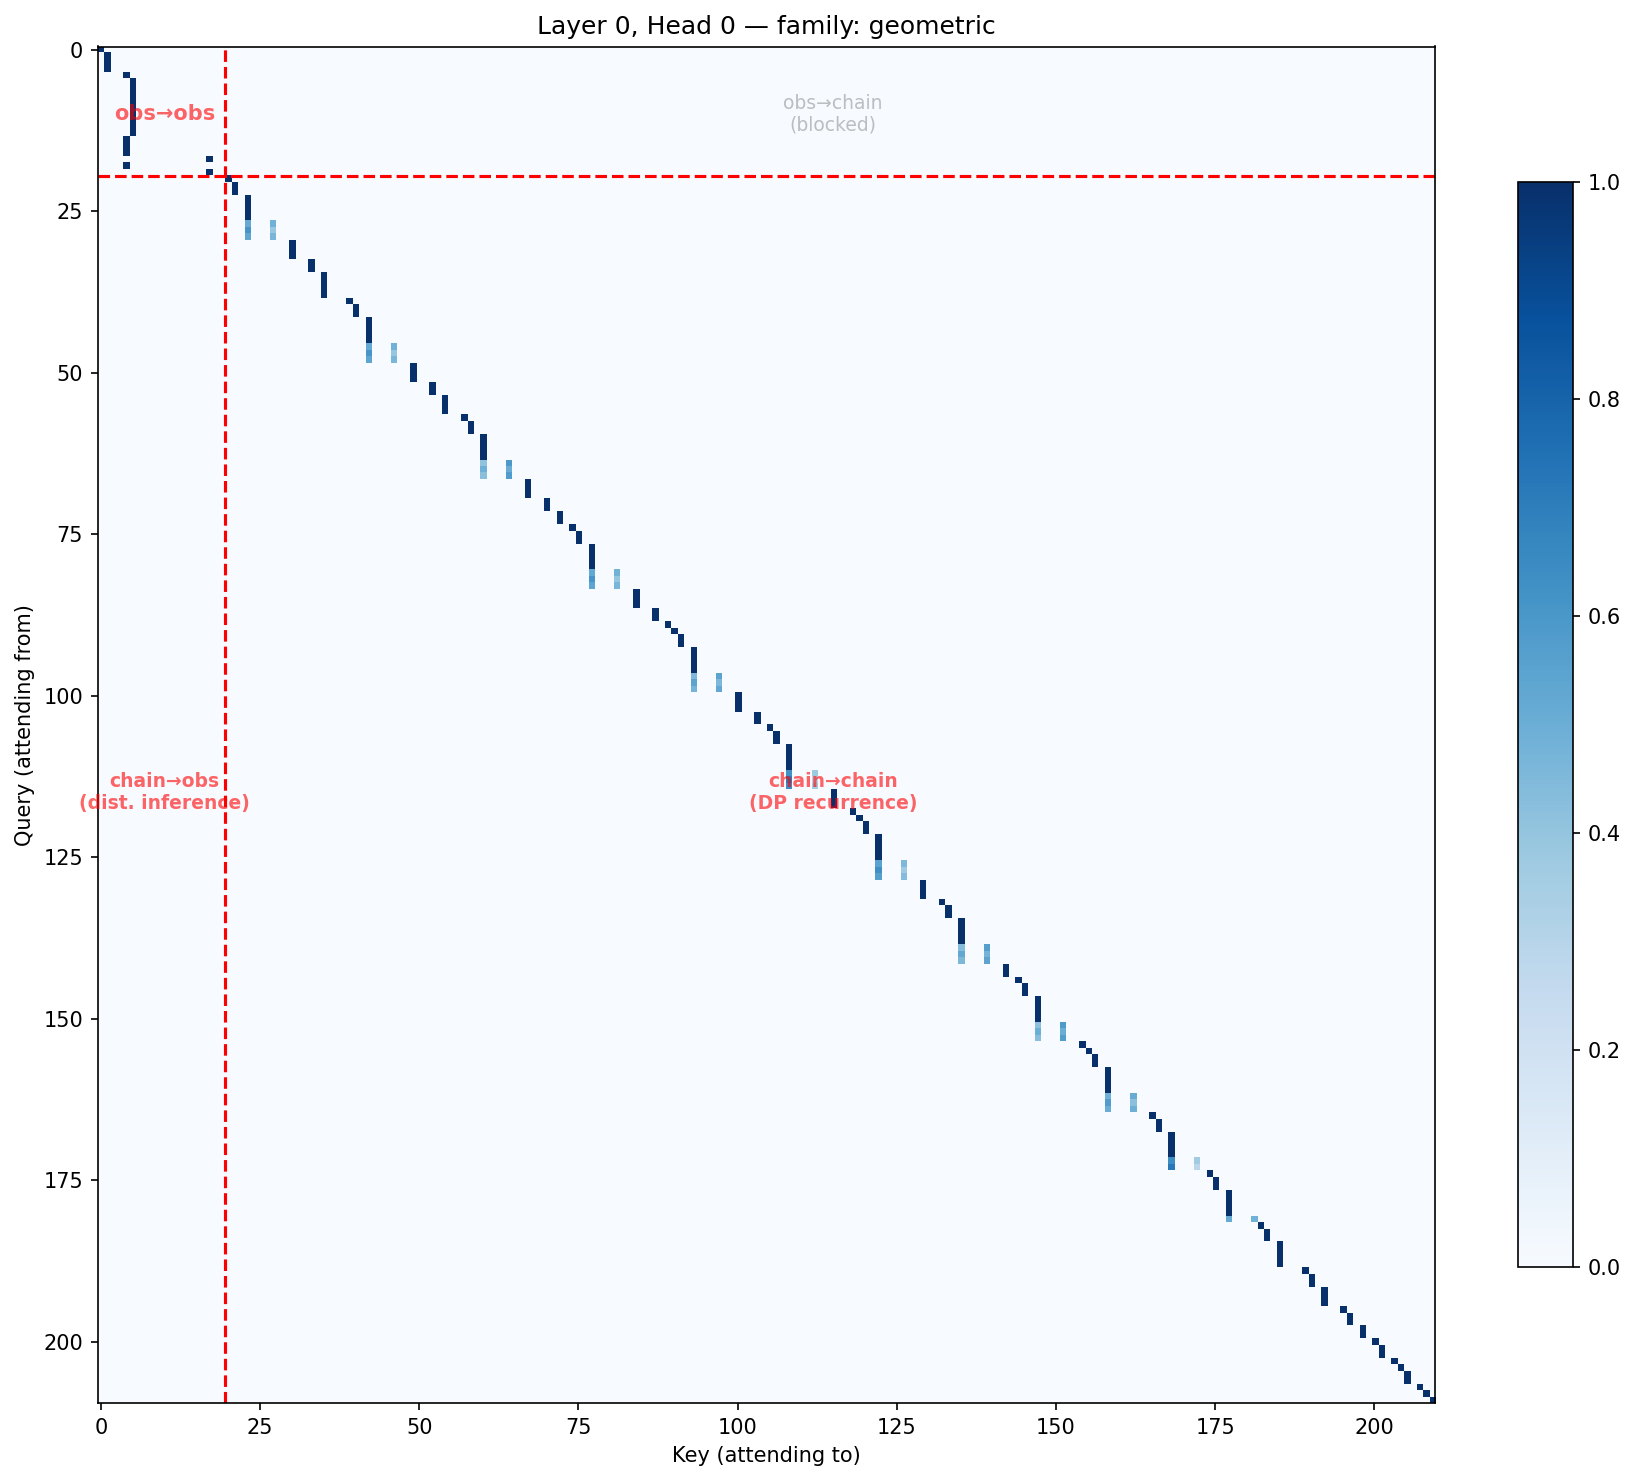
\includegraphics[width=0.48\linewidth]{plots/exp3_attention/attention_value+action/full_L0_H0_inst0.png}
\hfill
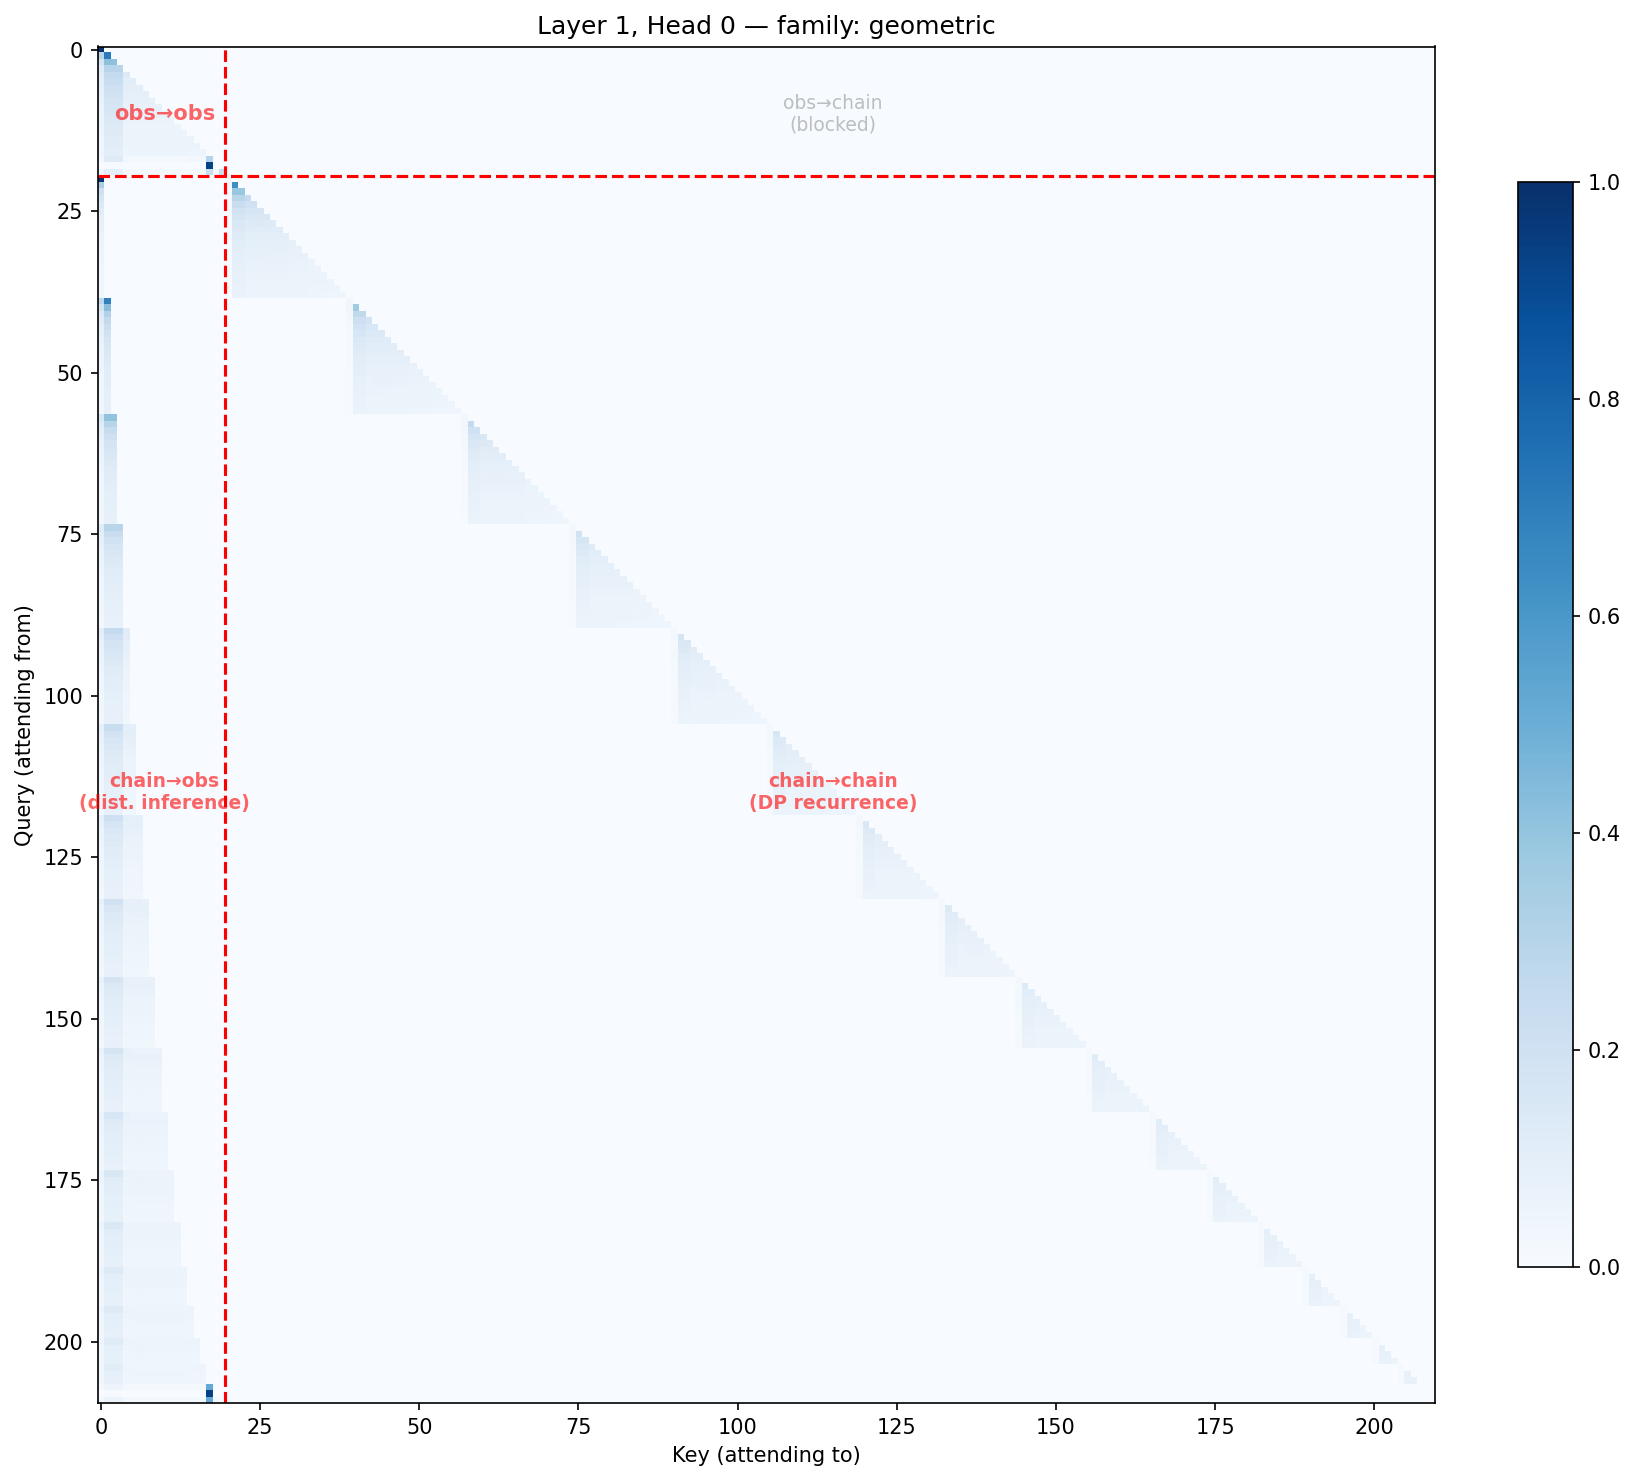
\includegraphics[width=0.48\linewidth]{plots/exp3_attention/attention_value+action/full_L1_H0_inst0.png}
\caption{Full attention maps (geometric family, $n=20$). Layer~0 (left): chain$\to$chain diagonal (DP recurrence). Layer~1 (right): chain$\to$obs diffuse (distribution inference).}
\label{fig:attn-full}
\end{figure}

The head specialization plot (Figure~\ref{fig:attn-head}) confirms layer-level specialization: Layer~0 heads attend almost entirely to chain tokens (green), while Layer~1 Head~0 increasingly reads observations (blue) at later decision steps where the posterior is more informative. This matches the Proposition~1 construction where Layer~1 (FFN) computes ReLU terms from the previous chain value and Layer~2 (attention) computes the PMF-weighted sum.

\begin{figure}[h]
\centering
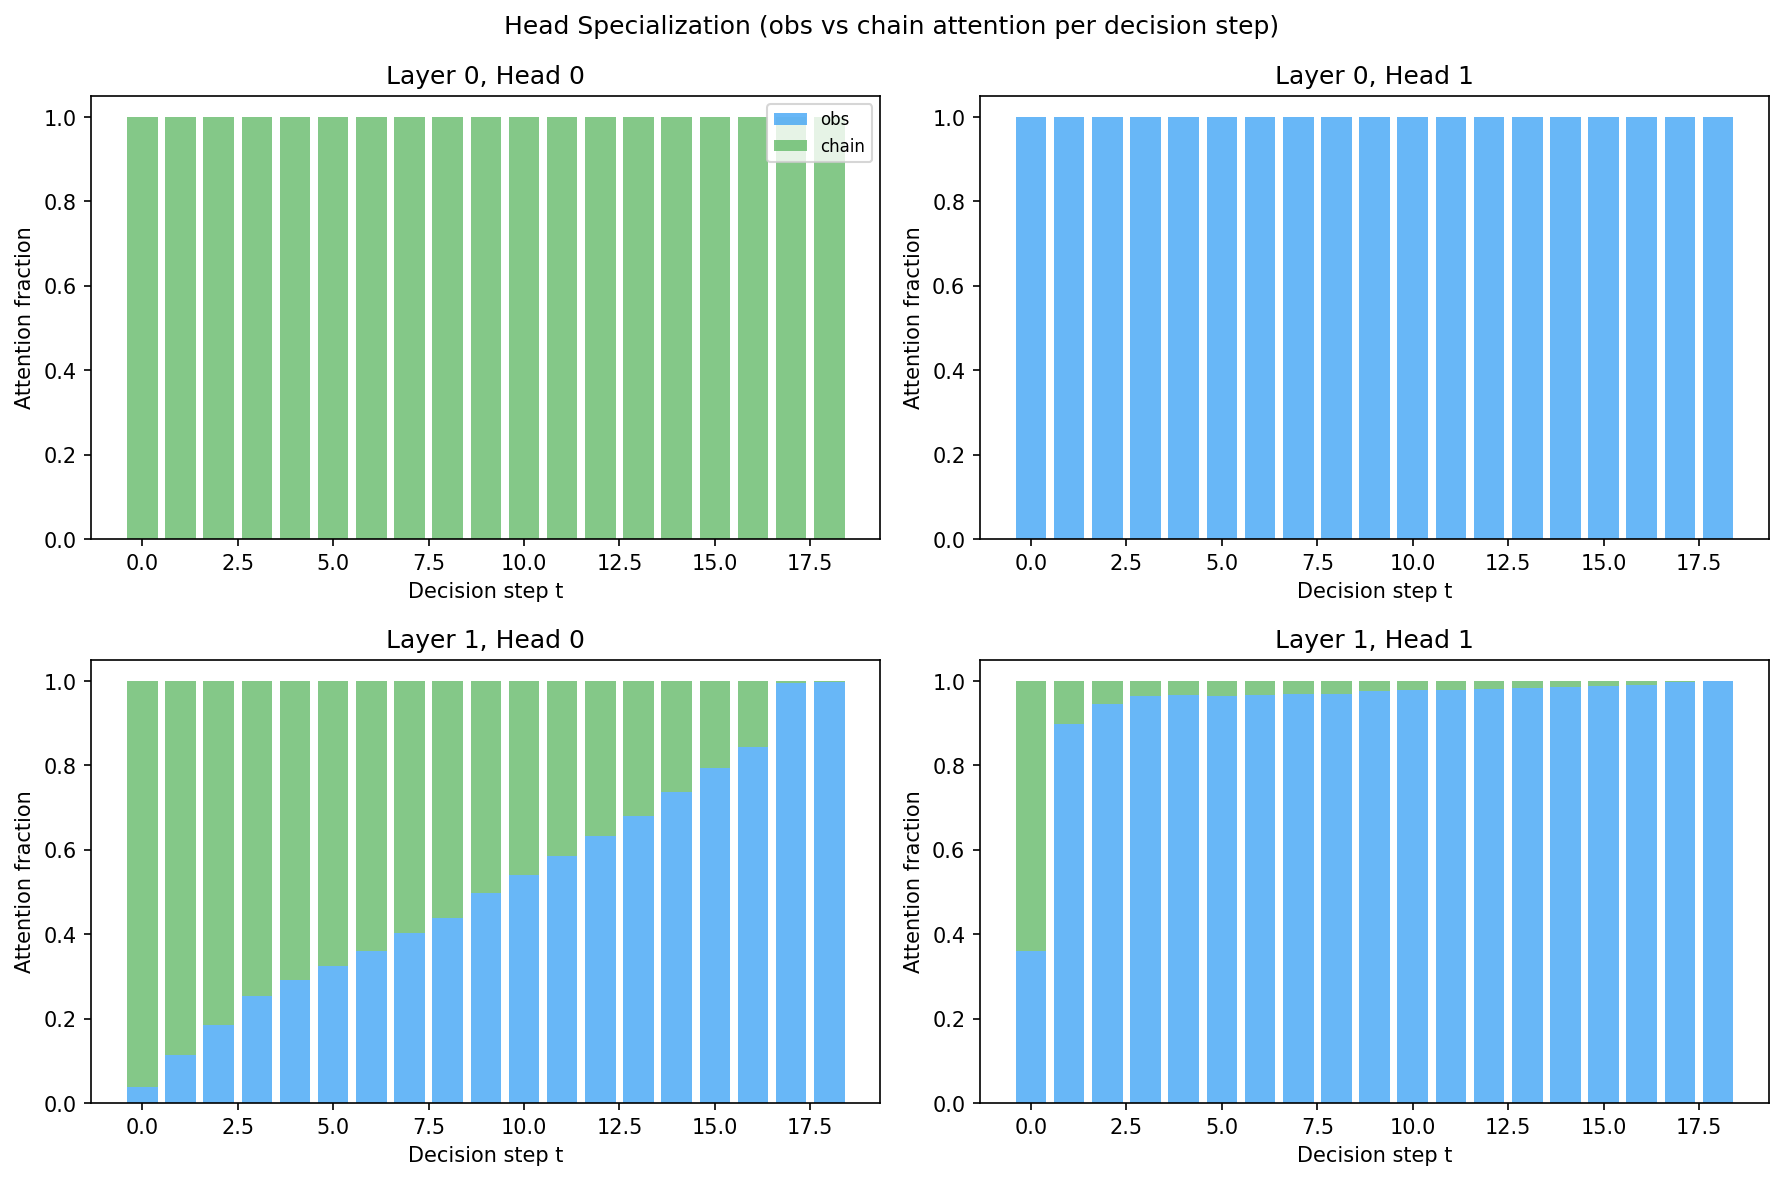
\includegraphics[width=0.48\linewidth]{plots/exp3_attention/attention_value+action/head_specialization_inst0.png}
\hfill
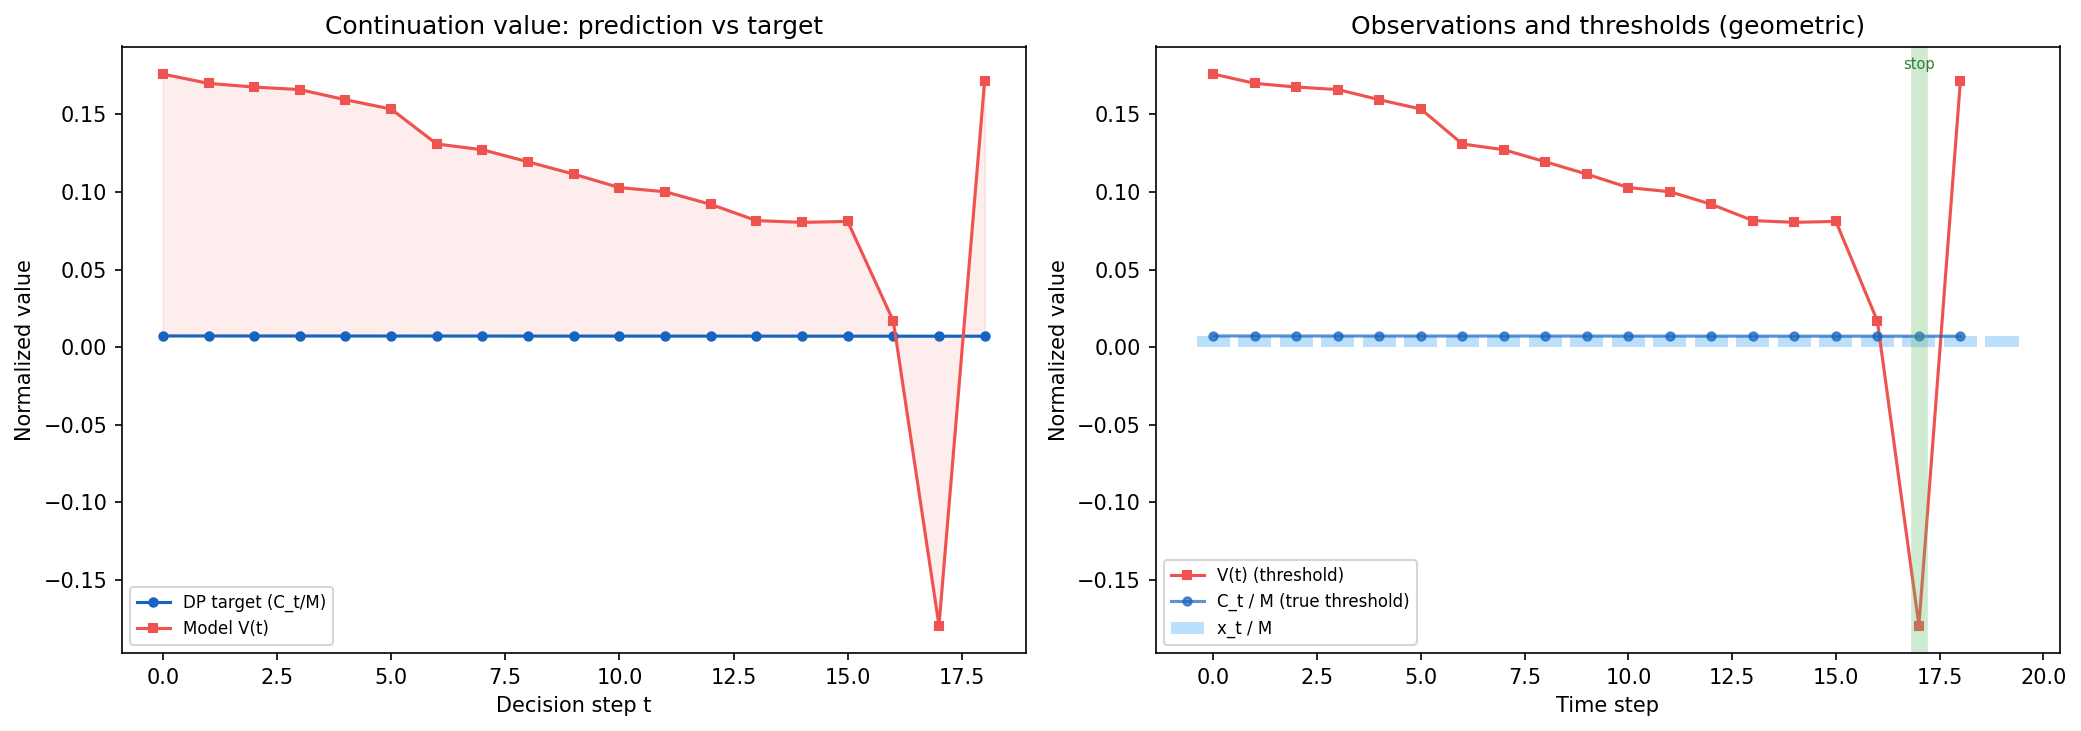
\includegraphics[width=0.48\linewidth]{plots/exp3_attention/attention_value+action/predictions_inst0.png}
\caption{Head specialization (left) and prediction accuracy (right). Geometric family, $n=20$.}
\label{fig:attn-head}
\end{figure}

The sub-chain internal attention (Figure~\ref{fig:attn-sub}) zooms into one sub-chain's within-chain pattern: Head~0 shows strong nearest-neighbor attention (each step reads the previous), while Head~1 attends more broadly. The observation profiles show that at later decision steps (more observations), attention distributes more uniformly---as expected for estimating a PMF from a growing sample.

\begin{figure}[h]
\centering
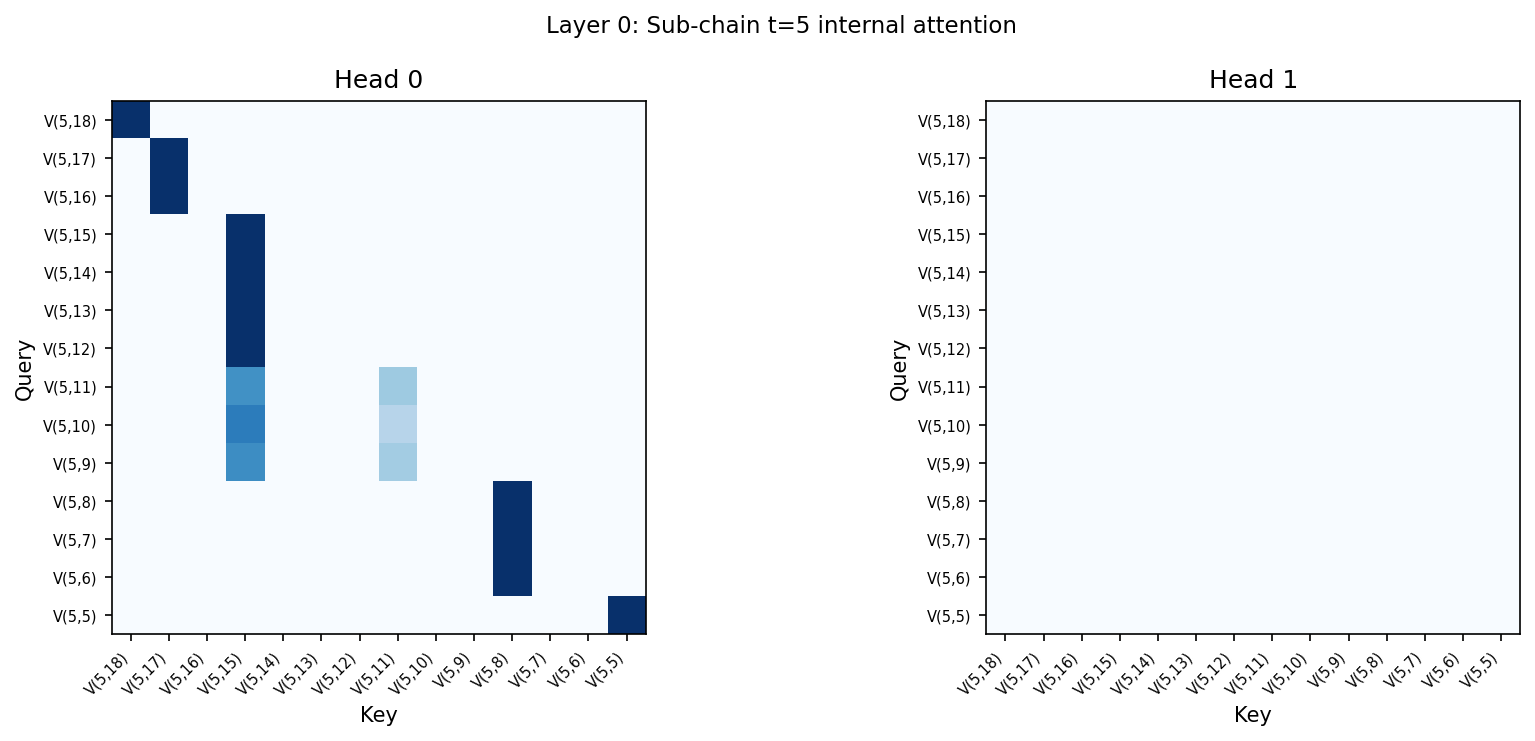
\includegraphics[width=0.48\linewidth]{plots/exp3_attention/attention_value+action/subchain_t5_L0_inst0.png}
\hfill
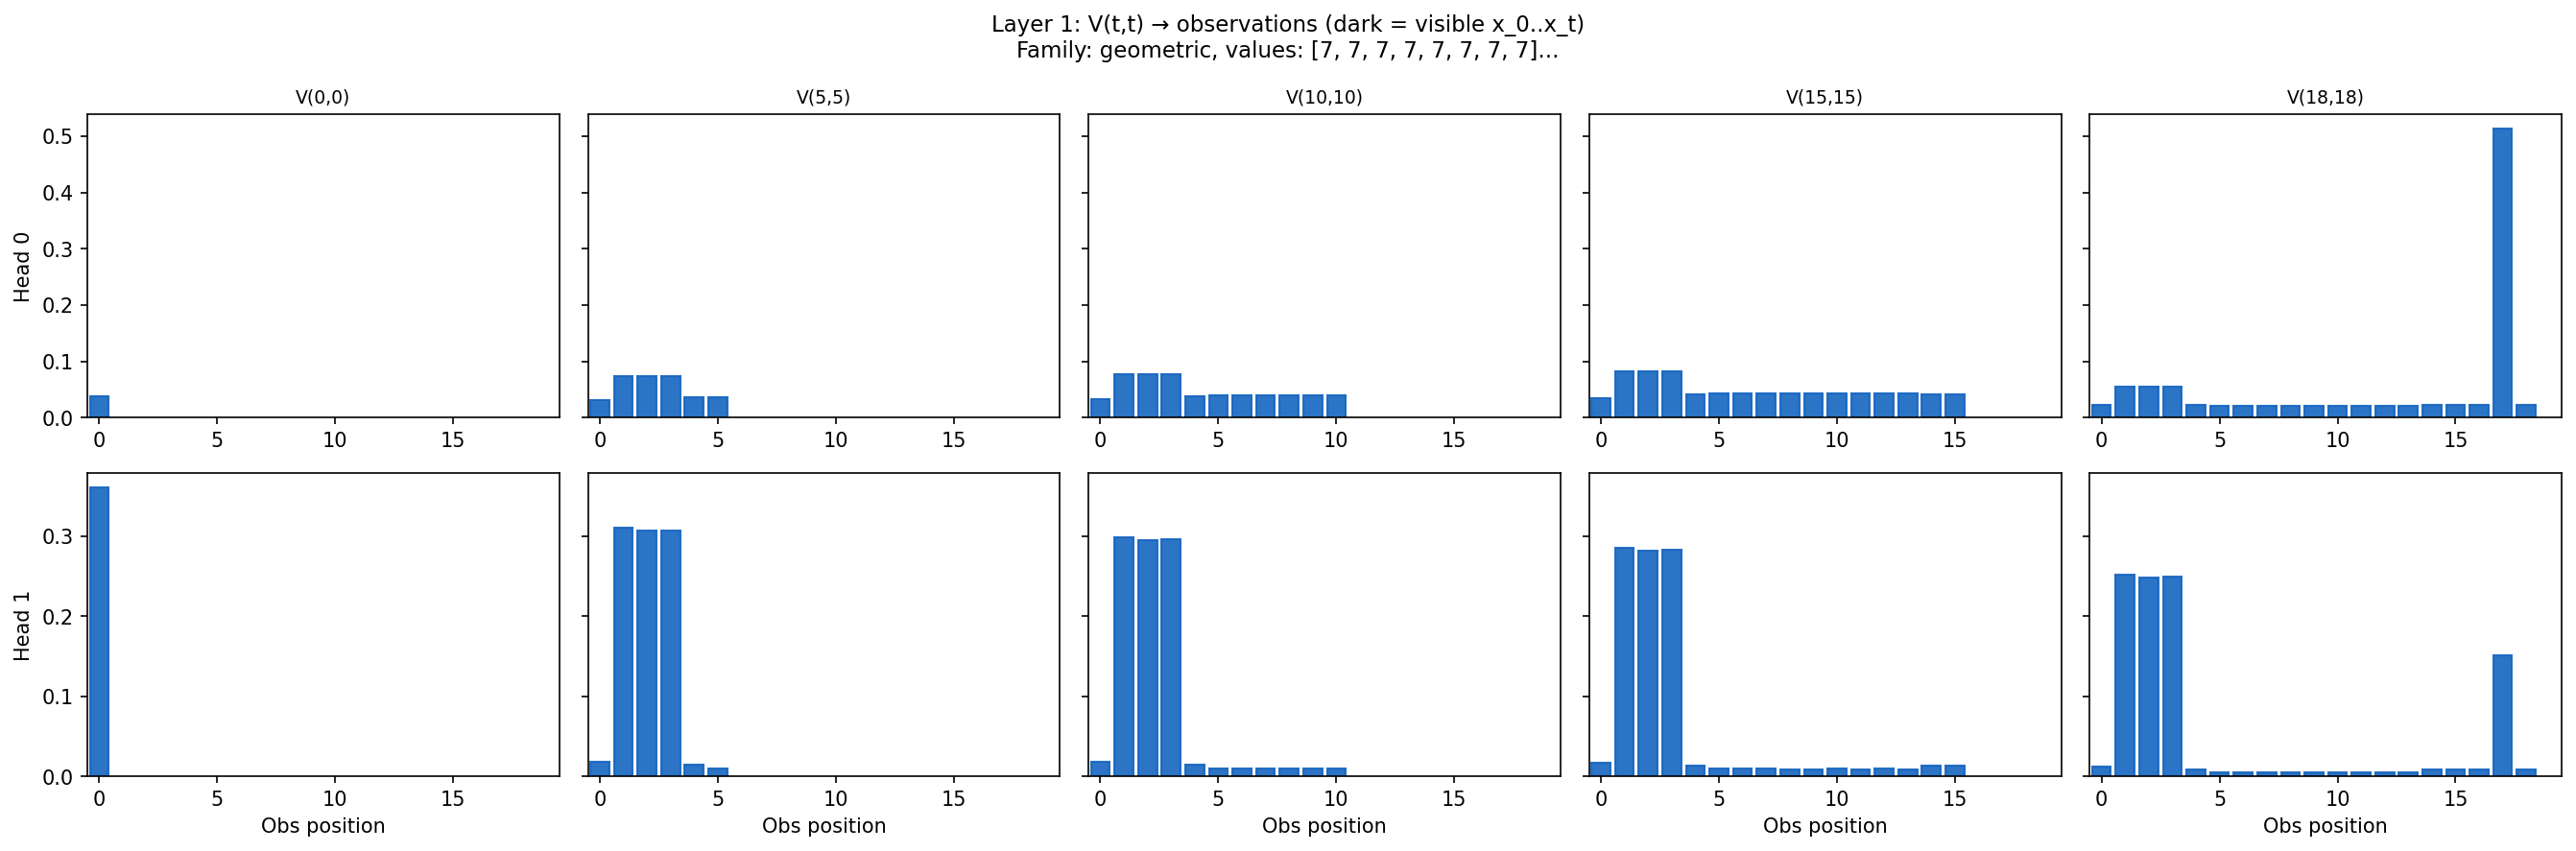
\includegraphics[width=0.48\linewidth]{plots/exp3_attention/attention_value+action/decision_obs_L1_inst0.png}
\caption{Sub-chain $t{=}5$ internal attention in Layer~0 (left). Decision step observation profiles in Layer~1 (right). Geometric family, $n=20$.}
\label{fig:attn-sub}
\end{figure}
